Έστω οι παραδοχές του προβλήματος ??. Έστω επιπλέον ότι $\hat{\bm{l}} =
\bm{l}$, δηλαδή μόνο ο προσανατολισμός του αισθητήρα πρέπει να εκτιμηθεί. Τότε
ας υπολογιστεί η εικονική σάρωση $\mathcal{S}_V$ μέσω δεσμοβολής (raycasting)
από την εκτίμηση $\hat{\bm{p}}$ στον χάρτη $\bm{M}$. Η εκτίμηση της περιστροφής
της εικονικής σάρωσης $\mathcal{S}_V$ σε σχέση με την πραγματική σάρωση
$\mathcal{S}_R$ μπορεί να βρεθεί μέσω των μεθόδων που παρουσιάζονται στις
ενότητες \ref{subsection:02_04_02:01}, \ref{subsection:02_04_02:02}, και
\ref{subsection:02_04_02:03}. Το σφάλμα της εκτίμησης προσανατολισμού μπορεί να
μειωθεί περαιτέρω μέσω της μεθόδου που παρουσιάζεται στην ενότητα
\ref{subsection:02_04_02:06}.

Στα συμφραζόμενα του παρόντος κεφαλαίου, έστω $\mathcal{F}\{\mathcal{S}\}$ ο
διακριτός μετασχηματισμός Fourier του σήματος $\mathcal{S}$,
$\mathcal{F}^{-1}\{\mathcal{S}\}$ ο αντίστροφός του, $\bm{c}^\ast$ ο συζυγής
του μιγαδικού αριθμού $\bm{c}$, $|\bm{c}|$ το μέτρο του, και $i$ η φανταστική
μονάδα.

%%%%%%%%%%%%%%%%%%%%%%%%%%%%%%%%%%%%%%%%%%%%%%%%%%%%%%%%%%%%%%%%%%%%%%%%%%%%%%%%
\subsection{Η μέθοδος Fourier-Mellin σε μία διάσταση}
\label{subsection:02_04_02:01}

Έστω ότι ο χώρος δειγματοληπτείται αρκετά πυκνά γωνιακά, τότε για
$k,\xi \in \mathbb{Z}_{\geq 0}$: $k,\xi \in [0, N_s-1]$:
\begin{align}
  \mathcal{S}_V[k] &\simeq \mathcal{S}_R[(k - \xi) \mod N_s] \Rightarrow \nonumber \\
  \mathcal{F}\{\mathcal{S}_V\}(u) &\simeq e^{-i 2\pi \xi u / N_s} \cdot \mathcal{F}\{\mathcal{S}_R\}(u) \nonumber
\end{align}
και, επομένως, αφού $2\pi \dfrac{\xi}{N_s} = \xi \dfrac{2\pi}{N_s} = \xi \gamma$,
όπου $\gamma$ είναι η διακριτική γωνία του αισθητήρα:
\begin{align}
  Q_{\mathcal{S}_V, \mathcal{S}_R}(u) & \triangleq \dfrac{\mathcal{F}\{\mathcal{S}_V\}^{\ast} \cdot \mathcal{F}\{\mathcal{S}_R\}}{|\mathcal{F}\{\mathcal{S}_V\}| \cdot |\mathcal{F}\{\mathcal{S}_R\}|} \nonumber \\
  &\simeq \dfrac{e^{-i \xi \gamma u} \cdot \mathcal{F}\{\mathcal{S}_R\}^\ast \cdot \mathcal{F}\{\mathcal{S}_R\}}{|e^{- i \xi \gamma u} \cdot \mathcal{F}\{\mathcal{S}_R\}^\ast | \cdot | \mathcal{F}\{\mathcal{S}_R\}|} \nonumber \\
  &= e^{-i \xi \gamma u} \cdot \dfrac{\mathcal{F}\{\mathcal{S}_R\}^\ast \cdot \mathcal{F}\{\mathcal{S}_R\}}{|\mathcal{F}\{\mathcal{S}_R\} | \cdot | \mathcal{F}\{\mathcal{S}_R\}|} \nonumber \\
  &= e^{-i \xi \gamma u}
  \label{eq:Q0}
\end{align}

Συνεπώς ο αντίστροφος διακριτός μετασχηματισμός Fourier του
$Q_{\mathcal{S}_V, \mathcal{S}_R}$ είναι μία Kronecker $\delta$-συνάρτηση
$q_{\mathcal{S}_V, \mathcal{S}_R} = \mathcal{F}^{-1}\{Q_{\mathcal{S}_V, \mathcal{S}_R}\}$
με κέντρο $\xi$:
\begin{align}
  \xi = \operatorname*{arg\,max}\limits_u \ q_{\mathcal{S}_V, \mathcal{S}_R}(u)
\end{align}

Η παραπάνω μέθοδος εκτίμησης του προσανατολισμού της στάσης
$\bm{p}(x,y,\theta)$ ονομάζεται στο εξής μέθοδος Fourier-Mellin σε μία
διάσταση.  Ο αλγόριθμος \ref{alg:algorithm_fmrc} παρουσιάζει σε ψευδοκώδικα τη
διαδικασία διόρθωσης προσανατολισμού με βάση την εν λόγω μέθοδο.

\begin{algorithm}
  \caption{\texttt{rc\_fm}}
  \begin{spacing}{1.3}
  \begin{algorithmic}[1]
    \REQUIRE $\bm{M}$, $\mathcal{S}_R$, $\mathcal{S}_V$, $\hat{\bm{p}}(x, y, \hat{\theta})$, $\gamma$, $N_s$
    \ENSURE $\hat{\theta}^\prime$, $q_{\max}$
    %\STATE $\mathcal{S}_V \leftarrow \texttt{scan\_map}(\bm{M}, \hat{\bm{p}}, N_s)$
    \STATE $q_{\mathcal{S}_V, \mathcal{S}_R} \leftarrow \mathcal{F}^{-1}\{Q_{\mathcal{S}_V, \mathcal{S}_R}\}$ (εξ. \ref{eq:Q0})
    \STATE $\xi = \operatorname*{arg\,max} \ q_{\mathcal{S}_V, \mathcal{S}_R}$
    \STATE $q_{\max} \leftarrow q_{\mathcal{S}_V, \mathcal{S}_R}[\xi] = \max q_{\mathcal{S}_V, \mathcal{S}_R}$
    \STATE $\hat{\theta}^\prime \leftarrow \hat{\theta} + \xi \gamma$
    \RETURN $(\hat{\theta}^\prime, q_{\max})$
  \end{algorithmic}
  \end{spacing}
  \label{alg:algorithm_fmrc}
\end{algorithm}


\begin{gg_box}
\begin{remark}
  \label{remark:02_04_02:01}
  Εάν η διαφορά του προσανατολισμού μεταξύ των στάσεων από τις οποίες ελήφθησαν οι
  σαρώσεις $\mathcal{S}_R$ και $\mathcal{S}_V$ είναι $\Delta\theta$, τότε
  $\Delta\theta = \xi\gamma + \delta\theta$, όπου $\mod(|\delta\theta|, \gamma) =
  \phi \in [0,\gamma/2]$. Επομένως, για δεδομένο αριθμό εκπεμπόμενων ακτίνων
  $N_s$ (ισοδύναμα, για δεδομένη διακριτική γωνία $\gamma$), ενημερώνοντας την
  εκτίμηση προσανατολισμού σε $\hat{\theta}^\prime$:
  \begin{align}
    \hat{\theta}^\prime = \hat{\theta} + \xi \gamma \label{eq:update_t1}
  \end{align}
  οδηγεί σε ένα επίλοιπο σφάλμα προσανατολισμού $\phi$:
  \begin{align}
    |\phi| \leq \dfrac{\gamma}{2}  \label{eq:phi_1}
  \end{align}
\end{remark}
\end{gg_box}

\begin{figure}[h]\centering
  \definecolor{sr}{RGB}{43,131,186}
\definecolor{svi}{RGB}{215,25, 28}
\definecolor{svf}{RGB}{179,143,59}
\definecolor{g}{RGB}{0,178,93}
\definecolor{k}{RGB}{0,0,0}

% GNUPLOT: LaTeX picture with Postscript
\begingroup
  \makeatletter
  \providecommand\color[2][]{%
    \GenericError{(gnuplot) \space\space\space\@spaces}{%
      Package color not loaded in conjunction with
      terminal option `colourtext'%
    }{See the gnuplot documentation for explanation.%
    }{Either use 'blacktext' in gnuplot or load the package
      color.sty in LaTeX.}%
    \renewcommand\color[2][]{}%
  }%
  \providecommand\includegraphics[2][]{%
    \GenericError{(gnuplot) \space\space\space\@spaces}{%
      Package graphicx or graphics not loaded%
    }{See the gnuplot documentation for explanation.%
    }{The gnuplot epslatex terminal needs graphicx.sty or graphics.sty.}%
    \renewcommand\includegraphics[2][]{}%
  }%
  \providecommand\rotatebox[2]{#2}%
  \@ifundefined{ifGPcolor}{%
    \newif\ifGPcolor
    \GPcolorfalse
  }{}%
  \@ifundefined{ifGPblacktext}{%
    \newif\ifGPblacktext
    \GPblacktexttrue
  }{}%
  % define a \g@addto@macro without @ in the name:
  \let\gplgaddtomacro\g@addto@macro
  % define empty templates for all commands taking text:
  \gdef\gplfronttext{}%
  \gdef\gplfronttext{}%
  \makeatother
  \ifGPblacktext
    % no textcolor at all
    \def\colorrgb#1{}%
    \def\colorgray#1{}%
  \else
    % gray or color?
    \ifGPcolor
      \def\colorrgb#1{\color[rgb]{#1}}%
      \def\colorgray#1{\color[gray]{#1}}%
      \expandafter\def\csname LTw\endcsname{\color{white}}%
      \expandafter\def\csname LTb\endcsname{\color{black}}%
      \expandafter\def\csname LTa\endcsname{\color{black}}%
      \expandafter\def\csname LT0\endcsname{\color[rgb]{1,0,0}}%
      \expandafter\def\csname LT1\endcsname{\color[rgb]{0,1,0}}%
      \expandafter\def\csname LT2\endcsname{\color[rgb]{0,0,1}}%
      \expandafter\def\csname LT3\endcsname{\color[rgb]{1,0,1}}%
      \expandafter\def\csname LT4\endcsname{\color[rgb]{0,1,1}}%
      \expandafter\def\csname LT5\endcsname{\color[rgb]{1,1,0}}%
      \expandafter\def\csname LT6\endcsname{\color[rgb]{0,0,0}}%
      \expandafter\def\csname LT7\endcsname{\color[rgb]{1,0.3,0}}%
      \expandafter\def\csname LT8\endcsname{\color[rgb]{0.5,0.5,0.5}}%
    \else
      % gray
      \def\colorrgb#1{\color{black}}%
      \def\colorgray#1{\color[gray]{#1}}%
      \expandafter\def\csname LTw\endcsname{\color{white}}%
      \expandafter\def\csname LTb\endcsname{\color{black}}%
      \expandafter\def\csname LTa\endcsname{\color{black}}%
      \expandafter\def\csname LT0\endcsname{\color{black}}%
      \expandafter\def\csname LT1\endcsname{\color{black}}%
      \expandafter\def\csname LT2\endcsname{\color{black}}%
      \expandafter\def\csname LT3\endcsname{\color{black}}%
      \expandafter\def\csname LT4\endcsname{\color{black}}%
      \expandafter\def\csname LT5\endcsname{\color{black}}%
      \expandafter\def\csname LT6\endcsname{\color{black}}%
      \expandafter\def\csname LT7\endcsname{\color{black}}%
      \expandafter\def\csname LT8\endcsname{\color{black}}%
    \fi
  \fi
    \setlength{\unitlength}{0.0500bp}%
    \ifx\gptboxheight\undefined%
      \newlength{\gptboxheight}%
      \newlength{\gptboxwidth}%
      \newsavebox{\gptboxtext}%
    \fi%
    \setlength{\fboxrule}{0.5pt}%
    \setlength{\fboxsep}{1pt}%
\begin{picture}(8000.00,4000.00)%
    \gplgaddtomacro\gplfronttext{%
    }%
    \gplgaddtomacro\gplfronttext{%
    }%
    \gplgaddtomacro\gplfronttext{%
      \colorrgb{0.15,0.15,0.15}%
      \put(4868,400){\makebox(0,0)[r]{\strut{}$2^{-2}$}}%
      \colorrgb{0.15,0.15,0.15}%
      \put(4868,755){\makebox(0,0)[r]{\strut{}$2^{-1}$}}%
      \colorrgb{0.15,0.15,0.15}%
      \put(4868,1111){\makebox(0,0)[r]{\strut{}$2^{0}$}}%
      \colorrgb{0.15,0.15,0.15}%
      \put(4868,1466){\makebox(0,0)[r]{\strut{}$2^{1}$}}%
      \colorrgb{0.15,0.15,0.15}%
      \put(4868,1822){\makebox(0,0)[r]{\strut{}$2^{2}$}}%
      \colorrgb{0.15,0.15,0.15}%
      \put(4868,2177){\makebox(0,0)[r]{\strut{}$2^{3}$}}%
      \colorrgb{0.15,0.15,0.15}%
      \put(4868,2533){\makebox(0,0)[r]{\strut{}$2^{4}$}}%
      \colorrgb{0.15,0.15,0.15}%
      \put(4868,2888){\makebox(0,0)[r]{\strut{}$2^{5}$}}%
      \colorrgb{0.15,0.15,0.15}%
      \put(4868,3244){\makebox(0,0)[r]{\strut{}$2^{6}$}}%
      \colorrgb{0.15,0.15,0.15}%
      \put(4868,3599){\makebox(0,0)[r]{\strut{}$2^{7}$}}%
      \colorrgb{0.15,0.15,0.15}%
      \put(5180,180){\makebox(0,0){\strut{}$1$}}%
      \colorrgb{0.15,0.15,0.15}%
      \put(5900,180){\makebox(0,0){\strut{}$5$}}%
      \colorrgb{0.15,0.15,0.15}%
      \put(6799,180){\makebox(0,0){\strut{}$10$}}%
    }%
    \gplgaddtomacro\gplfronttext{%
      \colorrgb{0.15,0.15,0.15}%
      \put(5400,3919){\makebox(0,0){\strut{}{\color{k}{\rule[0.6mm]{0.5cm}{0.5mm}}} $|\theta-\hat{\theta}[k]|/\gamma$}}%
      \put(6800,3919){\makebox(0,0){\strut{}{\color{g}{\rule[0.6mm]{0.5cm}{0.5mm}}} $2^{-1}$}}%
      \put(5899,-150){\makebox(0,0){\strut{}Αριθμός επαναλήψεων $k$}}%

      \put(1100,3919){\makebox(0,0){\strut{}{\color{k}{\rule[0.6mm]{0.5cm}{0.5mm}}} $\bm{M}$}}%
      \put(1850,3919){\makebox(0,0){\strut{}{\color{sr}{\rule[0.6mm]{0.5cm}{0.5mm}}} $\bm{p}$}}%
      \put(2600,3919){\makebox(0,0){\strut{}{\color{svi}{\rule[0.6mm]{0.5cm}{0.5mm}}} $\hat{\bm{p}}[0]$}}%
      \put(3500,3919){\makebox(0,0){\strut{}{\color{svf}{\rule[0.6mm]{0.5cm}{0.5mm}}} $\hat{\bm{p}}[1]$}}%
    }%
    \put(0,0){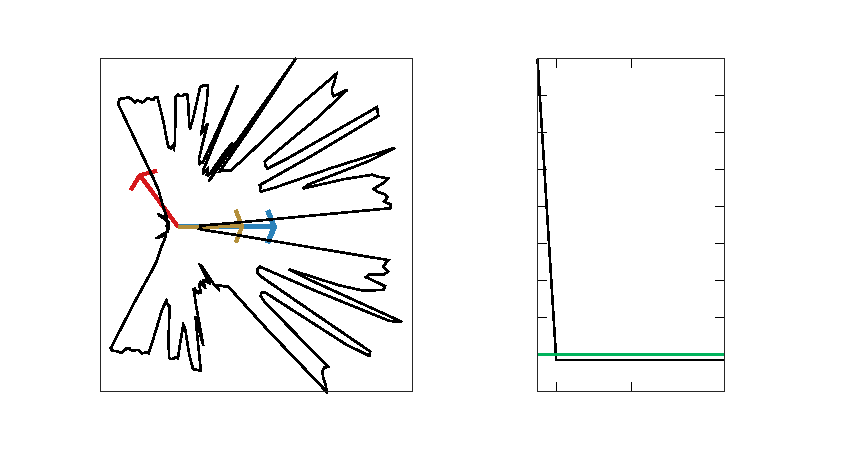
\includegraphics{./figures/parts/02/chapters/04/sections/02/rc_fm}}%
    \gplfronttext
  \end{picture}%
\endgroup

  \vspace{0.5cm}
  \caption{}
  \label{fig:}
\end{figure}


%%%%%%%%%%%%%%%%%%%%%%%%%%%%%%%%%%%%%%%%%%%%%%%%%%%%%%%%%%%%%%%%%%%%%%%%%%%%%%%%
\subsection{Η μέθοδος πρώτων αρχών}
\label{subsection:02_04_02:02}

Έστω μία δισδιάστατη σάρωση $\mathcal{S}$ που έχει ληφθεί από τη στάση
$(x,y,\theta)$ σε κάποιο σύστημα συντεταγμένων (ορισμός \ref{def:lidar}). Έστω
ότι το γωνιακό εύρος της $\mathcal{S}$ είναι $\lambda = 2\pi$. Οι συντεταγμένες
του τελικού σημείου της $n$-οστής ακτίνας της $\mathcal{S}$,
$n=0,1,\dots,N_s-1$, στο σύστημα συντεταγμένων είναι $(x_n,y_n)$:
\begin{align}
  x_n &= x + d_n \cos(\theta + \frac{2 \pi n}{N_s} - \pi) = -d_n \cos(\theta + \frac{2 \pi n}{N_s}) \label{eq:x_n}\\
  y_n &= y + d_n \sin(\theta + \frac{2 \pi n}{N_s} - \pi) = -d_n \sin(\theta + \frac{2 \pi n}{N_s}) \label{eq:y_n}
\end{align}
Εδώ παρατηρούμε ότι $-(x_n-x)$ και $(y_n-y)$ είναι αντίστοιχα το πραγματικό και
το φανταστικό μέρος της μιγαδικής ποσότητας
\begin{align}
  d_n e^{-i(\theta + \frac{2 \pi n}{N_s})} &= d_n \cos(\theta + \frac{2 \pi n}{N_s}) - i \cdot d_n \sin(\theta + \frac{2 \pi n}{N}) \nonumber \\
                                         &\leftstackrel{(\ref{eq:x_n}),(\ref{eq:y_n})}{=} -(x_n-x) + i \cdot (y_n-y) \label{eq:dne_complex_x_y}
\end{align}
και, επομένως
\begin{align}
  d_n e^{-i 2 \pi n/N_s} &= e^{i\theta}(-(x_n-x) + i \cdot (y_n-y)) \label{eq:dne_complex}
\end{align}
Αθροίζοντας την εξίσωση (\ref{eq:dne_complex}) επί του συνόλου των $N_s$
ακτίνων λαμβάνουμε τον πρώτο όρο του διακριτού μετασχηματισμού Fourier
του σήματος $\{d_n\}$, $n=0,1,\dots,N_s-1$:
\begin{align}
  \mathcal{F}\{\mathcal{S}\} = \sum\limits_{n=0}^{N_s-1}d_n \cdot e^{-i 2 \pi n/N_s} \ &\leftstackrel{(\ref{eq:dne_complex})}{=} \ \sum\limits_{n=0}^{N_s-1} e^{i\theta}(-(x_n-x) + i \cdot (y_n-y)) \nonumber  \\
           &= e^{i\theta} \sum\limits_{n=0}^{N_s-1} [ (x- i \cdot y) + (-x_n + i \cdot y_n) ]\nonumber \\
           &= e^{i\theta} N_s (x-i\cdot y) - e^{i\theta}\Delta \label{eq:F1}
\end{align}
όπου $\Delta \triangleq \sum\limits_{n=0}^{N_s-1} (x_n -i \cdot y_n)$.

Συμβολίζοντας με το γράμμα $R$ τις ποσότητες που αντιστοιχούν στην πραγματική
σάρωση $\mathcal{S}_R$, η οποία έχει ληφθεί από τη στάση του φυσικού αισθητήρα
$\bm{p}(x,y,\theta)$, και με $V$ εκείνες που αντιστοιχούν στην εικονική σάρωση
$\mathcal{S}_V$, η οποία έχει ληφθεί από τη στάση
$\hat{\bm{p}}(x,y,\hat{\theta})$:
\begin{align}
  \mathcal{F}\{\mathcal{S}_R\} &= \sum\limits_{n=0}^{N_s-1}d_n^R \cdot e^{-i 2 \pi n/N_s} \stackrel{(\ref{eq:F1})}{=} N_s e^{i\theta}(x-i\cdot y) - e^{i\theta} \Delta_R \label{eq:dne_complex_r} \\
  \mathcal{F}\{\mathcal{S}_V\} &= \sum\limits_{n=0}^{N_s-1}d_n^V \cdot e^{-i 2 \pi n/N_s} \stackrel{(\ref{eq:F1})}{=} N_s e^{i\hat{\theta}}(x-i\cdot y) - e^{i\hat{\theta}} \Delta_V \label{eq:dne_complex_v}
\end{align}

Έστω τώρα ότι
\begin{align}
  \Delta_R - \Delta_V &= \sum\limits_{n=0}^{N_s-1}(x_n^R-x_n^V) - i \cdot \sum\limits_{n=0}^{N_s-1}(y_n^R-y_n^V) \nonumber \\
                      &= N_s (\delta_x - i \cdot \delta_y)
\end{align}
όπου
\begin{align}
  \delta_x &\triangleq \frac{1}{N_s}\sum\limits_{n=0}^{N_s-1}(x_n^R-x_n^V) \label{eq:delta_x}\\
  \delta_y &\triangleq \frac{1}{N_s}\sum\limits_{n=0}^{N_s-1}(y_n^R-y_n^V) \label{eq:delta_y}
\end{align}
τότε
\begin{align}
  \Delta_V &= \Delta_R -N_s(\delta_x - i \cdot \delta_y) \label{eq:Delta_V_eq_Delta_R}
\end{align}

Ο πρώτος όρος του διακριτού μετασχηματισμού Fourier του σήματος που
αποτελείται από τη διαφορά των δύο σημάτων (\ref{eq:dne_complex_r}) και
(\ref{eq:dne_complex_v}) είναι:
\begin{align}
  \mathcal{F}\{\mathcal{S}_R\} - \mathcal{F}\{\mathcal{S}_V\} &= \sum\limits_{n=0}^{N_s-1}(d_n^R - d_n^V) \cdot e^{-i 2 \pi n/N_s} \nonumber \\
           &\leftstackrel{(\ref{eq:dne_complex_r}),(\ref{eq:dne_complex_v})}{=} N_s (x-i \cdot y)(e^{i\theta}-e^{i\hat{\theta}}) -e^{i\theta}\Delta_R+e^{i\hat{\theta}}\Delta_V \nonumber \\
          &\leftstackrel{(\ref{eq:Delta_V_eq_Delta_R})}{=} N_s (x-i \cdot y)(e^{i\theta}-e^{i\hat{\theta}}) -e^{i\theta}\Delta_R +e^{i\hat{\theta}}(\Delta_R -N_s(\delta_x - i \cdot \delta_y)) \nonumber \\
          &= N_s (x-i \cdot y)(e^{i\theta}-e^{i\hat{\theta}}) - \Delta_R (e^{i\theta}-e^{i\hat{\theta}})- N_s e^{i\hat{\theta}}(\delta_x - i\cdot \delta_y) \nonumber \\
          &= (e^{i\theta}-e^{i\hat{\theta}}) [N_s(x-i\cdot y) - \Delta_R]- N_s e^{i\hat{\theta}}(\delta_x - i\cdot \delta_y) \nonumber   \\
          &\leftstackrel{(\ref{eq:dne_complex_r})}{=} (e^{i\theta}-e^{i\hat{\theta}}) \dfrac{\mathcal{F}\{\mathcal{S}_R\}}{e^{i\theta}}- N_s e^{i\hat{\theta}}(\delta_x - i\cdot \delta_y) \nonumber \\
          &= (1-e^{-i(\theta-\hat{\theta})}) \mathcal{F}\{\mathcal{S}_R\}- N_s e^{i\hat{\theta}}(\delta_x - i\cdot \delta_y) \nonumber
\end{align}
άρα
\begin{align}
  -\mathcal{F}\{\mathcal{S}_V\} &= -e^{-i(\theta-\hat{\theta})} \mathcal{F}\{\mathcal{S}_R\}- N_s e^{i\hat{\theta}}(\delta_x - i\cdot \delta_y) \nonumber \\
  e^{-i(\theta-\hat{\theta})} &= \dfrac{\mathcal{F}\{\mathcal{S}_V\}}{\mathcal{F}\{\mathcal{S}_R\}} - \dfrac{N_s e^{i\hat{\theta}}}{\mathcal{F}\{\mathcal{S}_R\}}(\delta_x - i\cdot \delta_y) \nonumber
\end{align}
Χρησιμοποιώντας την πολική αναπαράσταση $\bm{A} = |\bm{A}| e^{i\angle \bm{A}}$:
\begin{align}
  e^{-i(\theta-\hat{\theta})} &= \dfrac{|\mathcal{F}\{\mathcal{S}_V\}|}{|\mathcal{F}\{\mathcal{S}_R\}|} e^{i(\angle \mathcal{F}\{\mathcal{S}_V\} - \angle \mathcal{F}\{\mathcal{S}_R\})} - \dfrac{e^{i(\hat{\theta}-\angle \mathcal{F}\{\mathcal{S}_R\})}}{|\mathcal{F}\{\mathcal{S}_R\}|} (N_s \delta_x - i\cdot N_s \delta_y) \label{eq:x1_final_big_eq}
\end{align}

Λόγω του γεγονότος ότι ο προσανατολισμός $\theta$ του αισθητήρα είναι άγνωστος,
τα τελικά σημεία $\{(x_n^R,y_n^R)\}$ καθίστανται ομοίως άγνωστα, και συνεπώς
και οι ποσότητες $\delta_x, \delta_y$. Προκειμένου να αποκτήσουμε μια αρχική
διαίσθηση ως προς τα μέτρα των τελευταίων κάνουμε την παρατήρηση ότι, εξ
ορισμού, οι ποσότητες $N_s \delta_x$ και $N_s \delta_y$ ποσοτικοποιούν τη
διαφορά της προσέγγισης των επικαμπύλιων ολοκληρωμάτων επί των καμπύλων που
ορίζουν τα τελικά σημεία των δύο σαρώσεων στους δύο κύριους άξονες $x$ και $y$.
Η προσέγγιση αυτή οφείλεται στο πεπερασμένο μέγεθος των εκπεμπόμενων ακτίνων
$N_s$. Επομένως υπό τις υποθέσεις ότι (α) ο χάρτης του περιβάλλοντος είναι
τέλεια αναπαράστασή του και (β) οι μετρήσεις του φυσικού αισθητήρα δεν
επηρεάζονται από διαταραχές: καθώς $N_s \rightarrow \infty$, $N_s \delta_x$,
$N_s \delta_y$ $\rightarrow 0$, τα οποία με τη σειρά τους σημαίνουν λόγω της
εξίσωσης (\ref{eq:x1_final_big_eq}) ότι
$\dfrac{|\mathcal{F}\{\mathcal{S}_V\}|}{|\mathcal{F}\{\mathcal{S}_R\}|} \rightarrow 1$
και $\theta-\hat{\theta} \rightarrow \angle \mathcal{F}\{\mathcal{S}_R\} - \angle \mathcal{F}\{\mathcal{S}_V\}$.

Η παραπάνω μέθοδος εκτίμησης του προσανατολισμού της στάσης $\bm{p}(x,y,\theta)$
ονομάζεται στο εξής μέθοδος πρώτων αρχών. Ο αλγόριθμος \ref{alg:algorithm_x1rc}
παρουσιάζει σε ψευδοκώδικα τη διαδικασία διόρθωσης προσανατολισμού με βάση την
εν λόγω μέθοδο.

\begin{algorithm}
  \caption{\texttt{rc\_x1}}
  \begin{spacing}{1.3}
  \begin{algorithmic}[1]
    \REQUIRE $\bm{M}$, $\mathcal{S}_R$, $\mathcal{S}_V$, $\hat{\bm{p}}(x, y, \hat{\theta})$, $\gamma$, $N_s$
    \ENSURE $\hat{\theta}^\prime$
    %\STATE $\mathcal{S}_V \leftarrow \texttt{scan\_map}(\bm{M}, \hat{\bm{p}}, N_s)$
    \STATE $\bm{R} = \mathcal{F}\{\mathcal{S}_R\}$
    \STATE $\bm{V} = \mathcal{F}\{\mathcal{S}_V\}$
    \STATE $\hat{\theta}^\prime \leftarrow \hat{\theta} + \arg(\bm{R}) - \arg(\bm{V})$
    \RETURN $\hat{\theta}^\prime$
  \end{algorithmic}
  \end{spacing}
  \label{alg:algorithm_x1rc}
\end{algorithm}


\begin{gg_box}
\begin{remark}
  \label{remark:02_04_02:02}
  Ενημερώνοντας την εκτίμηση προσανατολισμού σε $\hat{\theta}^\prime$:
  \begin{align}
  \hat{\theta}^\prime = \hat{\theta} + \angle \mathcal{F}\{\mathcal{S}_R\} - \angle\mathcal{F}\{\mathcal{S}_V\}
    \label{eq:update_t2}
  \end{align}
  οδηγεί σε ένα επίλοιπο σφάλμα προσανατολισμού $\phi$:
  \begin{align}
    \phi &= \tan^{-1}\dfrac{N_s \delta_x \tan(\theta - \angle \mathcal{F}\{\mathcal{S}_R\}) - N_s \delta_y}{|\mathcal{F}\{\mathcal{S}_R\}| + N_s \delta_x + N_s \delta_y \tan(\theta - \angle \mathcal{F}\{\mathcal{S}_R\})} \label{eq:phi2}
  \end{align}
  του οποίου το μέτρο είναι αντιστρόφως ανάλογο του αριθμού των ακτίνων $N_s$ που
  εκπέμπει ο αισθητήρας στην περίπτωση που τόσο η πραγματική μέτρηση
  $\mathcal{S}_R$ όσο και η εικονική σάρωση $\mathcal{S}_V$ δεν διαταράσσονται
  από θόρυβο.
\end{remark}
\end{gg_box}

\begin{figure}[h]\centering
  \definecolor{sr}{RGB}{43,131,186}
\definecolor{svi}{RGB}{215,25, 28}
\definecolor{svf}{RGB}{179,143,59}
\definecolor{g}{RGB}{0,178,93}
\definecolor{k}{RGB}{0,0,0}

% GNUPLOT: LaTeX picture with Postscript
\begingroup
  \makeatletter
  \providecommand\color[2][]{%
    \GenericError{(gnuplot) \space\space\space\@spaces}{%
      Package color not loaded in conjunction with
      terminal option `colourtext'%
    }{See the gnuplot documentation for explanation.%
    }{Either use 'blacktext' in gnuplot or load the package
      color.sty in LaTeX.}%
    \renewcommand\color[2][]{}%
  }%
  \providecommand\includegraphics[2][]{%
    \GenericError{(gnuplot) \space\space\space\@spaces}{%
      Package graphicx or graphics not loaded%
    }{See the gnuplot documentation for explanation.%
    }{The gnuplot epslatex terminal needs graphicx.sty or graphics.sty.}%
    \renewcommand\includegraphics[2][]{}%
  }%
  \providecommand\rotatebox[2]{#2}%
  \@ifundefined{ifGPcolor}{%
    \newif\ifGPcolor
    \GPcolorfalse
  }{}%
  \@ifundefined{ifGPblacktext}{%
    \newif\ifGPblacktext
    \GPblacktexttrue
  }{}%
  % define a \g@addto@macro without @ in the name:
  \let\gplgaddtomacro\g@addto@macro
  % define empty templates for all commands taking text:
  \gdef\gplfronttext{}%
  \gdef\gplfronttext{}%
  \makeatother
  \ifGPblacktext
    % no textcolor at all
    \def\colorrgb#1{}%
    \def\colorgray#1{}%
  \else
    % gray or color?
    \ifGPcolor
      \def\colorrgb#1{\color[rgb]{#1}}%
      \def\colorgray#1{\color[gray]{#1}}%
      \expandafter\def\csname LTw\endcsname{\color{white}}%
      \expandafter\def\csname LTb\endcsname{\color{black}}%
      \expandafter\def\csname LTa\endcsname{\color{black}}%
      \expandafter\def\csname LT0\endcsname{\color[rgb]{1,0,0}}%
      \expandafter\def\csname LT1\endcsname{\color[rgb]{0,1,0}}%
      \expandafter\def\csname LT2\endcsname{\color[rgb]{0,0,1}}%
      \expandafter\def\csname LT3\endcsname{\color[rgb]{1,0,1}}%
      \expandafter\def\csname LT4\endcsname{\color[rgb]{0,1,1}}%
      \expandafter\def\csname LT5\endcsname{\color[rgb]{1,1,0}}%
      \expandafter\def\csname LT6\endcsname{\color[rgb]{0,0,0}}%
      \expandafter\def\csname LT7\endcsname{\color[rgb]{1,0.3,0}}%
      \expandafter\def\csname LT8\endcsname{\color[rgb]{0.5,0.5,0.5}}%
    \else
      % gray
      \def\colorrgb#1{\color{black}}%
      \def\colorgray#1{\color[gray]{#1}}%
      \expandafter\def\csname LTw\endcsname{\color{white}}%
      \expandafter\def\csname LTb\endcsname{\color{black}}%
      \expandafter\def\csname LTa\endcsname{\color{black}}%
      \expandafter\def\csname LT0\endcsname{\color{black}}%
      \expandafter\def\csname LT1\endcsname{\color{black}}%
      \expandafter\def\csname LT2\endcsname{\color{black}}%
      \expandafter\def\csname LT3\endcsname{\color{black}}%
      \expandafter\def\csname LT4\endcsname{\color{black}}%
      \expandafter\def\csname LT5\endcsname{\color{black}}%
      \expandafter\def\csname LT6\endcsname{\color{black}}%
      \expandafter\def\csname LT7\endcsname{\color{black}}%
      \expandafter\def\csname LT8\endcsname{\color{black}}%
    \fi
  \fi
    \setlength{\unitlength}{0.0500bp}%
    \ifx\gptboxheight\undefined%
      \newlength{\gptboxheight}%
      \newlength{\gptboxwidth}%
      \newsavebox{\gptboxtext}%
    \fi%
    \setlength{\fboxrule}{0.5pt}%
    \setlength{\fboxsep}{1pt}%
\begin{picture}(8000.00,4000.00)%
    \gplgaddtomacro\gplfronttext{%
    }%
    \gplgaddtomacro\gplfronttext{%
    }%
    \gplgaddtomacro\gplfronttext{%
      \colorrgb{0.15,0.15,0.15}%
      \put(4868,647){\makebox(0,0)[r]{\strut{}$2^{-3}$}}%
      \colorrgb{0.15,0.15,0.15}%
      \put(4868,942){\makebox(0,0)[r]{\strut{}$2^{-2}$}}%
      \colorrgb{0.15,0.15,0.15}%
      \put(4868,1237){\makebox(0,0)[r]{\strut{}$2^{-1}$}}%
      \colorrgb{0.15,0.15,0.15}%
      \put(4868,1533){\makebox(0,0)[r]{\strut{}$2^{0}$}}%
      \colorrgb{0.15,0.15,0.15}%
      \put(4868,1828){\makebox(0,0)[r]{\strut{}$2^{1}$}}%
      \colorrgb{0.15,0.15,0.15}%
      \put(4868,2123){\makebox(0,0)[r]{\strut{}$2^{2}$}}%
      \colorrgb{0.15,0.15,0.15}%
      \put(4868,2418){\makebox(0,0)[r]{\strut{}$2^{3}$}}%
      \colorrgb{0.15,0.15,0.15}%
      \put(4868,2713){\makebox(0,0)[r]{\strut{}$2^{4}$}}%
      \colorrgb{0.15,0.15,0.15}%
      \put(4868,3009){\makebox(0,0)[r]{\strut{}$2^{5}$}}%
      \colorrgb{0.15,0.15,0.15}%
      \put(4868,3304){\makebox(0,0)[r]{\strut{}$2^{6}$}}%
      \colorrgb{0.15,0.15,0.15}%
      \put(4868,3599){\makebox(0,0)[r]{\strut{}$2^{7}$}}%
      \colorrgb{0.15,0.15,0.15}%
      \put(5180,180){\makebox(0,0){\strut{}$1$}}%
      \colorrgb{0.15,0.15,0.15}%
      \put(5900,180){\makebox(0,0){\strut{}$5$}}%
      \colorrgb{0.15,0.15,0.15}%
      \put(6799,180){\makebox(0,0){\strut{}$10$}}%
    }%
    \gplgaddtomacro\gplfronttext{%
      \colorrgb{0.15,0.15,0.15}%
      \put(5500,3819){\makebox(0,0){\strut{}{\color{k}{\rule[0.6mm]{0.5cm}{0.5mm}}} $|e_\theta|/\gamma$}}%
      \put(6500,3819){\makebox(0,0){\strut{}{\color{g}{\rule[0.6mm]{0.5cm}{0.5mm}}} $2^{-1}$}}%
      \put(5899,-150){\makebox(0,0){\strut{}Αριθμός επαναλήψεων}}%

      \put(1100,3819){\makebox(0,0){\strut{}{\color{k}{\rule[0.6mm]{0.5cm}{0.5mm}}} $\bm{M}$}}%
      \put(1850,3819){\makebox(0,0){\strut{}{\color{sr}{\rule[0.6mm]{0.5cm}{0.5mm}}} $\bm{p}$}}%
      \put(2600,3819){\makebox(0,0){\strut{}{\color{svi}{\rule[0.6mm]{0.5cm}{0.5mm}}} $\hat{\bm{p}}[0]$}}%
      \put(3500,3819){\makebox(0,0){\strut{}{\color{svf}{\rule[0.6mm]{0.5cm}{0.5mm}}} $\hat{\bm{p}}[10]$}}%
    }%
    \put(0,0){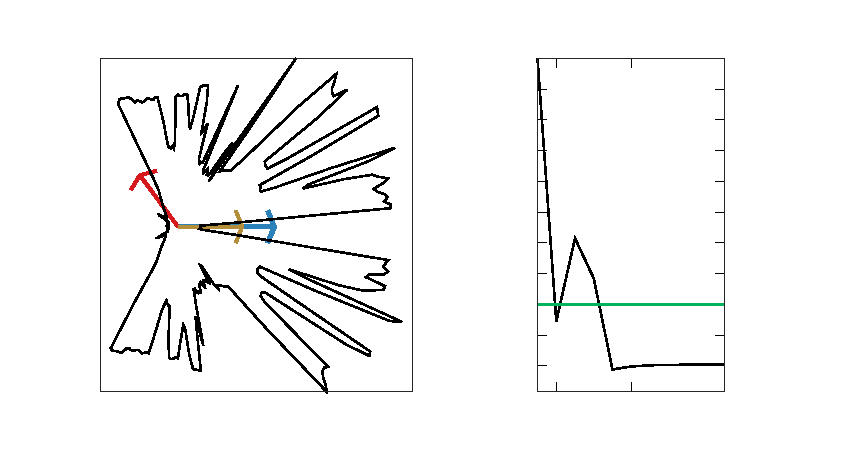
\includegraphics{./figures/parts/02/chapters/04/sections/02/rc_x1}}%
    \gplfronttext
  \end{picture}%
\endgroup

  \vspace{0.5cm}
  \caption{}
  \label{fig:}
\end{figure}

%%%%%%%%%%%%%%%%%%%%%%%%%%%%%%%%%%%%%%%%%%%%%%%%%%%%%%%%%%%%%%%%%%%%%%%%%%%%%%%%
\subsection{Η μέθοδος του Προκρούστη}
\label{subsection:02_04_02:03}

Έστω ότι η προβολή των τελικών σημείων των ακτίνων της σάρωσης $\mathcal{S}_V$
γύρω από τη στάση $\hat{\bm{p}}(x,y,\hat{\theta})$ παράγει το σύνολο σημείων
$\bm{P}_V$ στο οριζόντιο επίπεδο. Έστω ότι η ίδια προβολή για τη σάρωση
$\mathcal{S}_R$ ως προς τη στάση $\bm{p}(x,y,\theta)$ παράγει το σύνολο
$\bm{P}_R$. Η περιστροφή της στάσης $\hat{\bm{p}}$ που ευθυγραμμίζει βέλτιστα
το σύνολο σημείων $\bm{P}_V$ σε σχέση με το $\bm{P}_R$ μπορεί να βρεθεί από τη
λύση του Ορθογώνιου Προσκρούστειου προβλήματος \cite{Schonemann1966a} για
πίνακες εισόδου $\bm{P}_V$ και $\bm{P}_R$. Στην περίπτωση που ο πίνακας
μετασχηματισμού περιορίζεται στο να έχει τη δομή πίνακα περιστροφής $\bm{R}$:
$\det{(\bm{R})} = 1$, το πρόβλημα ευθυγράμμισης ονομάζεται Περιορισμένο
Ορθογώνιο Προσκρούστειο πρόβλημα. Η λύση του δίνεται στο \cite{Umeyama1991} και
περιγράφεται παρακάτω.

Δεδομένου ότι στα συμφραζόμενα του προβλήματός ?? μας η θέση $\bm{l}$ είναι
άγνωστη, τα τελικά σημεία κάθε σάρωσης λαμβάνονται με την προβολή κάθε σάρωσης
στο επίπεδο $x-y$ σύμφωνα με το τοπικό σύστημα αναφοράς της κάθεμίας, δηλαδή
σαν να είχε ληφθεί η κάθε μιά από το $O(0,0,0)$. Ο πίνακας περιστροφής $\bm{R}$
που ευθυγραμμίζει βέλτιστα το σύνολο $\bm{P}_V$ με το $\bm{P}_R$ είναι ο
πίνακας που ελαχιστοποιεί την απόκλιση των περιεστραμμένων σημείων
$\bm{R}\bm{P}_V$ από το $\bm{P}_R$:
\begin{align}
  \operatorname*{arg\,min}\limits_{\bm{R}} \|\bm{P}_R - \bm{R} \cdot \bm{P}_V\|_F^2 \nonumber
\end{align}
όπου $\|\bm{A}\|_F = (\bm{A}^\top\bm{A})^{1/2}$ δηλώνει το μέτρο Frobenius του
πίνακα πραγματικών τιμών $\bm{A}$. Έστω ο τελεστής $\text{tr}(\bm{A})$ ότι
δηλώνει το ίχνος του πίνακα $\bm{A}$. Τότε
\begin{align}
  \|\bm{P}_R - \bm{R} \bm{P}_V\|_F^2 = \text{tr}(\bm{P}_R^\top \bm{P}_R + \bm{P}_V^\top \bm{P}_V) - 2 \ \text{tr}(\bm{R} \bm{P}_R \bm{P}_V^\top)
  \label{eq:expanded_frob_norm}
\end{align}

Δεδομένου ότι μόνο ο δεύτερος όρος της δεξιάς πλευράς εξαρτάται από τον πίνακα
$\bm{R}$, για την ελαχιστοποίηση της (\ref{eq:expanded_frob_norm}) ως προς
$\bm{R}$ αρκεί να βρεθεί ο πίνακας περιστροφής $\bm{R}$ που μεγιστοποιεί
το ίχνος $\text{tr}(\bm{R} \bm{P}_V \bm{P}_R^\top)$. Ο βέλτιστος πίνακας
$\bm{R}$ δίνεται από το λήμμα \ref{lm:umeyama}:

\begin{lemma}
  \label{lm:umeyama}
  Έστω $\bm{P}_R$ και $\bm{P}_V$ πίνακες διαστάσεων $2 \times N_s$, $\bm{R}$
  πίνακας διαστάσεων $2 \times 2$, και $\bm{U} \bm{D} \bm{V}^\top$ η αποσύνθεση
  του $\bm{P}_R \bm{P}_V^\top$ σε ιδιάζουσες τιμές (Singular Value
  Decomposition---SVD). Τότε ο πίνακας $\bm{R}$ που ελαχιστοποιεί το μέτρο
  $\|\bm{P}_R - \bm{R} \cdot \bm{P}_V\|_F^2$ δίνεται από τη σχέση
  $\bm{R} = \bm{U} \bm{S} \bm{V}^\top$, όπου
  $\bm{S} = \text{diag}(1,\det{(\bm{U}\bm{V})})$.
\end{lemma}

\begin{corollary}
  \label{corollary:umeyama}
  Η τιμή του μέγιστου ίχνους
  $T(\bm{P}_R, \bm{P}_V) \triangleq \max\text{tr}(\bm{R} \bm{P}_R \bm{P}_V^\top)$
  είναι
  \begin{align}
  \max\text{tr}(\bm{R} \bm{P}_R \bm{P}_V^\top) = \text{tr}(\bm{D}\bm{S})
  \end{align}
\end{corollary}

Το λήμμα \ref{lm:umeyama} παρέχει τον βέλτιστο πίνακα περιστροφής $\bm{R}$ υπό
την προϋπόθεση ότι τόσο το σύνολο $\bm{P}_R$ όσο και το $\bm{P}_V$ είναι
γνωστά.  Ωστόσο, στα συμφραζόμενα του προβλήματος ?? τα τελικά σημεία
$\bm{P}_R$ υπολογίζονται από έναν αυθαίρετο προσανατολισμό επειδή ο επιθυμητός
προσανατολισμός είναι θεμελιωδώς άγνωστος. Επομένως ο υπολογισμός του πίνακα
$\bm{R}$ και η εξαγωγή  του σχετικού προσανατολισμού του $\bm{P}_V$ σε σχέση με
το $\bm{P}_R$ από τον πίνακα $\bm{R}$ \textit{σε ένα βήμα} είναι αδύνατη. Αυτό
που μπορεί να γίνει για την εκτίμηση του προσανατολισμού της στάσης $\bm{p}$ ως
προς τον προσανατολισμό της στάσης $\hat{\bm{p}}$ είναι το εξής. Υπολογίζεται
το γινόμενο $\bm{P}_R \bm{P}_V^\top$ σε $O(N_s^2)$, η αποσύνθεσή του σε
ιδιάζουσες τιμές σε $O(1)$, καταγράφεται η τιμή του ίχνους
$\text{tr}(\bm{D}\bm{S})$ σε $O(1)$, μετατοπίζεται ο πίνακας $\bm{P}_V$ κατά
στήλες προς τα αριστερά μία φορά, και επαναλαμβάνεται η διαδικασία $N_s-1$
φορές. Έστω ότι η επανάληψη $\psi \in \mathbb{Z}_{\geq 0}$ καταγράφει το
μέγιστο ίχνος: τότε η περιστροφή της στάσης $\hat{\bm{p}}$ κατά $\psi \gamma$
μεγιστοποιεί το ίχνος $\text{tr}(\bm{R} \bm{P}_R \bm{P}_V^\top)$ και
ελαχιστοποιεί το μέτρο του σφάλματος ευθυγράμμισης
(\ref{eq:expanded_frob_norm}) για μία δεδομένη διακριτική γωνία $\gamma$. Η
παραπάνω διαδικασία αποδίδει τη βέλτιστη περιστροφή επειδή το ίχνος
$\text{tr}(\bm{D}\bm{S})$ ουσιαστικά αναλαμβάνει το ρόλο ενός μέτρου
ευθυγράμμισης μεταξύ των συνόλων σημείων $\bm{P}_V$ και $\bm{P}_R$.

Η παραπάνω διαδικασία καταγραφής $N_s$ ιχνών μπορεί να υπολογιστεί είτε με ευθύ
τρόπο, πολυπλοκότητας $O(N_s^3)$, είτε μέσω με της μεθόδου που παρουσιάζεται
στο \cite{Dogan2015} με σημαντικά μειωμένη πολυπλοκότητα $O(N_s \log N_s)$.  Η
μέθοδος αυτή θα αναφέρεται στο εξής ως μέθοδος DBH και περιγράφεται παρακάτω.


Έστω $\widetilde{\bm{A}}$ ο πίνακας $\bm{A}$ με αντίστροφη σειρά στηλών,
$\bm{P}_R = [\bm{p}_R^x; \bm{p}_R^y]$,
$\widetilde{\bm{P}}_V = [\bm{p}_V^x; \bm{p}_V^y]$. Έστω επίσης ότι ο τελεστής
$\odot$ υποδηλώνει τον πολλαπλασιασμό κατά στοιχείο. Τότε υπολογίζονται
τέσσερα διανύσματα μεγέθους $N_s$:
\begin{align}
  \bm{m}_{11} = \mathcal{F}^{-1}\{ \mathcal{F}\{\bm{p}_R^x\} \odot \mathcal{F}\{\bm{p}_V^x\} \} \} \nonumber \\
  \bm{m}_{12} = \mathcal{F}^{-1}\{ \mathcal{F}\{\bm{p}_R^y\} \odot \mathcal{F}\{\bm{p}_V^x\} \} \} \nonumber \\
  \bm{m}_{21} = \mathcal{F}^{-1}\{ \mathcal{F}\{\bm{p}_R^x\} \odot \mathcal{F}\{\bm{p}_V^y\} \} \} \nonumber \\
  \bm{m}_{22} = \mathcal{F}^{-1}\{ \mathcal{F}\{\bm{p}_R^y\} \odot \mathcal{F}\{\bm{p}_V^y\} \} \} \nonumber
\end{align}
Μετά τον υπολογισμό των πινάκων $\bm{m}_{kl}$, $k,l = 1,2$, υπολογίζονται
$N_s$ πίνακες μεγέθους $2\times2$ σύμφωνα με:
\begin{align}
  \bm{M}_j =
  \begin{bmatrix}
    \bm{m}_{11}^j & \bm{m}_{12}^j \\
    \bm{m}_{21}^j & \bm{m}_{22}^j
  \end{bmatrix}
\end{align}
όπου $j = 0,\dots,N-1$, και $\bm{m}_{kl}^j$ είναι το $j$-οστό στοιχείο του
διανύσματος $\bm{m}_{kl}$. Ο πίνακας $\bm{M}_j$ είναι ίσος με τον πίνακα
$\bm{P}_R (\bm{P}_V^{N_s-1-j})^\top$, όπου ο συμβολισμός $\bm{A}^k$  δηλώνει
τον πίνακα $\bm{A}$ του οποίου οι στήλες έχουν μετατοπιστεί $k$ φορές προς τα
αριστερά. Η απόδειξη χρησιμοποιεί το θεώρημα κυκλικής συνέλιξης του DFT και
παραλείπεται.

Αφού υπολογιστούν και σχηματιστούν όλοι οι $N_s$ $\bm{M}_j$ πίνακες, κάθε ένας
αποσυντίθεται σε ιδιάζουσες τιμές. Το ίχνος κάθε πίνακα $\bm{R}_j \bm{M}_j$
καταγράφεται με την εφαρμογή του λήμματος \ref{lm:umeyama} και του επακόλουθου
\ref{corollary:umeyama}. Έστω ότι το μέγιστο ίχνος καταγράφεται για τον δείκτη
$J$, τότε η περιστροφή της στάσης $\hat{\bm{p}}$ κατά $(N_s-1-J)\gamma =
\psi\gamma$ επιτυγχάνει το ίδιο αποτέλεσμα με την ευθεία μέθοδο υψηλότερης
πολυπλοκότητας για μία δεδομένη διακριτική γωνία $\gamma$.

Η παραπάνω μέθοδος εκτίμησης του προσανατολισμού της στάσης
$\bm{p}(x,y,\theta)$ ονομάζεται στο εξής μέθοδος του Προκρούστη. Ο αλγόριθμος
\ref{alg:algorithm_x1rc} παρουσιάζει σε ψευδοκώδικα τη διαδικασία διόρθωσης
προσανατολισμού με βάση την εν λόγω μέθοδο. Ο αλγόριθμος
\ref{alg:algorithm_core_ufrc} παρουσιάζει σε ψευδοκώδικα τη μέθοδο DBH.

\begin{algorithm}[h]
  \caption{\texttt{rc\_uf}}
  \begin{spacing}{1.3}
  \begin{algorithmic}[1]
    \REQUIRE $\bm{M}$, $\mathcal{S}_R$, $\mathcal{S}_V$, $\hat{\bm{p}}(x, y, \hat{\theta})$, $\gamma$, $N_s$
    \ENSURE $\hat{\theta}^\prime$, $T$
    %\STATE $\mathcal{S}_V \leftarrow \texttt{scan\_map}(\bm{M}, \hat{\bm{p}}, N_s)$
    \STATE $\bm{P}_R \leftarrow \texttt{project}(\mathcal{S}_R, (0,0,0))$
    \STATE $\bm{P}_V \leftarrow \texttt{project}(\mathcal{S}_V, (0,0,0))$
    \STATE $(J,T) \leftarrow \texttt{rc\_uf\_core}(\bm{P}_R, \bm{P}_V)$ (Αλγόριθμος \ref{alg:algorithm_core_ufrc})
    \STATE $\psi = N_s - 1 - J$
    \STATE $\hat{\theta}^\prime \leftarrow \hat{\theta} + \psi \gamma$
    \RETURN $(\hat{\theta}^\prime, T)$
  \end{algorithmic}
  \end{spacing}
  \label{alg:algorithm_ufrc}
\end{algorithm}


\begin{algorithm}[h]
  \caption{\texttt{rc\_uf\_core}}
  \begin{spacing}{1.3}
  \begin{algorithmic}[1]
    \REQUIRE $\bm{P}_R$, $\bm{P}_V$
    \ENSURE $J$, $T(\bm{P}_R, \bm{P}_V)$
    \STATE \texttt{reverse}$(\bm{P}_V)$
    \STATE $\bm{p}_R^x \leftarrow \text{first row of } \bm{P}_R$
    \STATE $\bm{p}_R^y \leftarrow \text{second row of } \bm{P}_R$
    \STATE $\bm{p}_V^x \leftarrow \text{first row of } \bm{P}_V$
    \STATE $\bm{p}_V^y \leftarrow \text{second row of } \bm{P}_V$
    \STATE $\bm{m}_{11} \leftarrow \texttt{IDFT}(\texttt{DFT}(\bm{p}_R^x) \odot \texttt{DFT}(\bm{p}_V^x))$
    \STATE $\bm{m}_{12} \leftarrow \texttt{IDFT}(\texttt{DFT}(\bm{p}_R^y) \odot \texttt{DFT}(\bm{p}_V^x))$
    \STATE $\bm{m}_{21} \leftarrow \texttt{IDFT}(\texttt{DFT}(\bm{p}_R^x) \odot \texttt{DFT}(\bm{p}_V^y))$
    \STATE $\bm{m}_{22} \leftarrow \texttt{IDFT}(\texttt{DFT}(\bm{p}_R^y) \odot \texttt{DFT}(\bm{p}_V^y))$
    \STATE $\bm{T} \leftarrow \{\varnothing\}$
    \FOR{\texttt{$j = 0:N_s-1$}}
      \vspace{0.1cm}
      \STATE $\bm{M}_j \leftarrow
        \begin{bmatrix}
          \bm{m}_{11}(j) & \bm{m}_{12}(j) \\
          \bm{m}_{21}(j) & \bm{m}_{22}(j)
        \end{bmatrix}$
        \vspace{0.1cm}
        \STATE $(\bm{U}, \bm{D}, \bm{V}) \leftarrow \texttt{SVD}(\bm{M}_j)$
        \STATE \texttt{append} $\texttt{trace}(\bm{D} \cdot \texttt{diag}(1,\det(\bm{U}\bm{V})))$ to $\bm{T}$
    \ENDFOR
    \STATE \texttt{reverse}$(\bm{T})$
    \STATE $J \leftarrow \arg\max\bm{T}$
    \STATE $T_{\max} \leftarrow \max \{\bm{T}\} = \bm{T}[J]$
    \RETURN $(J,T_{\max})$
  \end{algorithmic}
  \end{spacing}
  \label{alg:algorithm_core_ufrc}
\end{algorithm}


\begin{gg_box}
\begin{remark}
  \label{remark:02_04_02:03}
  Εάν η διαφορά του προσανατολισμού μεταξύ των στάσεων από τις οποίες ελήφθησαν οι
  σαρώσεις $\mathcal{S}_R$ και $\mathcal{S}_V$ είναι $\Delta\theta$, τότε
  $\Delta\theta = (N_s-1-J)\gamma + \delta\theta$, όπου
  $\mod(|\delta\theta|, \gamma) = \phi \in [0,\gamma/2]$. Επομένως, για δεδομένο
  αριθμό εκπεμπόμενων ακτίνων $N_s$ (ισοδύναμα, για δεδομένη διακριτική γωνία
  $\gamma$), ενημερώνοντας την εκτίμηση προσανατολισμού σε $\hat{\theta}^\prime$:
  \begin{align}
    \hat{\theta}^\prime = \hat{\theta} + (N_s-1-J) \gamma \label{eq:update_t3}
  \end{align}
  οδηγεί σε ένα επίλοιπο σφάλμα προσανατολισμού $\phi$:
  \begin{align}
    |\phi| \leq \dfrac{\gamma}{2}  \label{eq:phi_3}
  \end{align}
\end{remark}
\end{gg_box}

\begin{figure}[h]\centering
  \definecolor{sr}{RGB}{43,131,186}
\definecolor{svi}{RGB}{215,25, 28}
\definecolor{svf}{RGB}{179,143,59}
\definecolor{g}{RGB}{0,178,93}
\definecolor{k}{RGB}{0,0,0}

% GNUPLOT: LaTeX picture with Postscript
\begingroup
  \makeatletter
  \providecommand\color[2][]{%
    \GenericError{(gnuplot) \space\space\space\@spaces}{%
      Package color not loaded in conjunction with
      terminal option `colourtext'%
    }{See the gnuplot documentation for explanation.%
    }{Either use 'blacktext' in gnuplot or load the package
      color.sty in LaTeX.}%
    \renewcommand\color[2][]{}%
  }%
  \providecommand\includegraphics[2][]{%
    \GenericError{(gnuplot) \space\space\space\@spaces}{%
      Package graphicx or graphics not loaded%
    }{See the gnuplot documentation for explanation.%
    }{The gnuplot epslatex terminal needs graphicx.sty or graphics.sty.}%
    \renewcommand\includegraphics[2][]{}%
  }%
  \providecommand\rotatebox[2]{#2}%
  \@ifundefined{ifGPcolor}{%
    \newif\ifGPcolor
    \GPcolorfalse
  }{}%
  \@ifundefined{ifGPblacktext}{%
    \newif\ifGPblacktext
    \GPblacktexttrue
  }{}%
  % define a \g@addto@macro without @ in the name:
  \let\gplgaddtomacro\g@addto@macro
  % define empty templates for all commands taking text:
  \gdef\gplfronttext{}%
  \gdef\gplfronttext{}%
  \makeatother
  \ifGPblacktext
    % no textcolor at all
    \def\colorrgb#1{}%
    \def\colorgray#1{}%
  \else
    % gray or color?
    \ifGPcolor
      \def\colorrgb#1{\color[rgb]{#1}}%
      \def\colorgray#1{\color[gray]{#1}}%
      \expandafter\def\csname LTw\endcsname{\color{white}}%
      \expandafter\def\csname LTb\endcsname{\color{black}}%
      \expandafter\def\csname LTa\endcsname{\color{black}}%
      \expandafter\def\csname LT0\endcsname{\color[rgb]{1,0,0}}%
      \expandafter\def\csname LT1\endcsname{\color[rgb]{0,1,0}}%
      \expandafter\def\csname LT2\endcsname{\color[rgb]{0,0,1}}%
      \expandafter\def\csname LT3\endcsname{\color[rgb]{1,0,1}}%
      \expandafter\def\csname LT4\endcsname{\color[rgb]{0,1,1}}%
      \expandafter\def\csname LT5\endcsname{\color[rgb]{1,1,0}}%
      \expandafter\def\csname LT6\endcsname{\color[rgb]{0,0,0}}%
      \expandafter\def\csname LT7\endcsname{\color[rgb]{1,0.3,0}}%
      \expandafter\def\csname LT8\endcsname{\color[rgb]{0.5,0.5,0.5}}%
    \else
      % gray
      \def\colorrgb#1{\color{black}}%
      \def\colorgray#1{\color[gray]{#1}}%
      \expandafter\def\csname LTw\endcsname{\color{white}}%
      \expandafter\def\csname LTb\endcsname{\color{black}}%
      \expandafter\def\csname LTa\endcsname{\color{black}}%
      \expandafter\def\csname LT0\endcsname{\color{black}}%
      \expandafter\def\csname LT1\endcsname{\color{black}}%
      \expandafter\def\csname LT2\endcsname{\color{black}}%
      \expandafter\def\csname LT3\endcsname{\color{black}}%
      \expandafter\def\csname LT4\endcsname{\color{black}}%
      \expandafter\def\csname LT5\endcsname{\color{black}}%
      \expandafter\def\csname LT6\endcsname{\color{black}}%
      \expandafter\def\csname LT7\endcsname{\color{black}}%
      \expandafter\def\csname LT8\endcsname{\color{black}}%
    \fi
  \fi
    \setlength{\unitlength}{0.0500bp}%
    \ifx\gptboxheight\undefined%
      \newlength{\gptboxheight}%
      \newlength{\gptboxwidth}%
      \newsavebox{\gptboxtext}%
    \fi%
    \setlength{\fboxrule}{0.5pt}%
    \setlength{\fboxsep}{1pt}%
\begin{picture}(8000.00,4000.00)%
    \gplgaddtomacro\gplfronttext{%
    }%
    \gplgaddtomacro\gplfronttext{%
    }%
    \gplgaddtomacro\gplfronttext{%
      \colorrgb{0.15,0.15,0.15}%
      \put(4868,400){\makebox(0,0)[r]{\strut{}$2^{-2}$}}%
      \colorrgb{0.15,0.15,0.15}%
      \put(4868,755){\makebox(0,0)[r]{\strut{}$2^{-1}$}}%
      \colorrgb{0.15,0.15,0.15}%
      \put(4868,1111){\makebox(0,0)[r]{\strut{}$2^{0}$}}%
      \colorrgb{0.15,0.15,0.15}%
      \put(4868,1466){\makebox(0,0)[r]{\strut{}$2^{1}$}}%
      \colorrgb{0.15,0.15,0.15}%
      \put(4868,1822){\makebox(0,0)[r]{\strut{}$2^{2}$}}%
      \colorrgb{0.15,0.15,0.15}%
      \put(4868,2177){\makebox(0,0)[r]{\strut{}$2^{3}$}}%
      \colorrgb{0.15,0.15,0.15}%
      \put(4868,2533){\makebox(0,0)[r]{\strut{}$2^{4}$}}%
      \colorrgb{0.15,0.15,0.15}%
      \put(4868,2888){\makebox(0,0)[r]{\strut{}$2^{5}$}}%
      \colorrgb{0.15,0.15,0.15}%
      \put(4868,3244){\makebox(0,0)[r]{\strut{}$2^{6}$}}%
      \colorrgb{0.15,0.15,0.15}%
      \put(4868,3599){\makebox(0,0)[r]{\strut{}$2^{7}$}}%
      \colorrgb{0.15,0.15,0.15}%
      \put(5180,180){\makebox(0,0){\strut{}$1$}}%
      \colorrgb{0.15,0.15,0.15}%
      \put(5900,180){\makebox(0,0){\strut{}$5$}}%
      \colorrgb{0.15,0.15,0.15}%
      \put(6799,180){\makebox(0,0){\strut{}$10$}}%
    }%
    \gplgaddtomacro\gplfronttext{%
      \colorrgb{0.00,0.00,0.00}%
      \put(5400,3919){\makebox(0,0){\strut{}{\color{k}{\rule[0.6mm]{0.5cm}{0.5mm}}} $\dfrac{|\theta-\hat{\theta}[k]|}{\gamma}$}}%
      \put(6800,3919){\makebox(0,0){\strut{}{\color{g}{\rule[0.6mm]{0.5cm}{0.5mm}}} $2^{-1}$}}%
      \put(5899,-150){\makebox(0,0){\strut{}Αριθμός επαναλήψεων $k$}}%
      \put(2300,-150){\makebox(0,0){\strut{}Προκρούστης}}%

      \put(1100,3919){\makebox(0,0){\strut{}{\color{k}{\rule[0.6mm]{0.5cm}{0.5mm}}} $\bm{M}$}}%
      \put(1850,3919){\makebox(0,0){\strut{}{\color{sr}{\rule[0.6mm]{0.5cm}{0.5mm}}} $\bm{p}$}}%
      \put(2600,3919){\makebox(0,0){\strut{}{\color{svi}{\rule[0.6mm]{0.5cm}{0.5mm}}} $\hat{\bm{p}}[0]$}}%
      \put(3500,3919){\makebox(0,0){\strut{}{\color{svf}{\rule[0.6mm]{0.5cm}{0.5mm}}} $\hat{\bm{p}}[1]$}}%

    }%
    \put(0,0){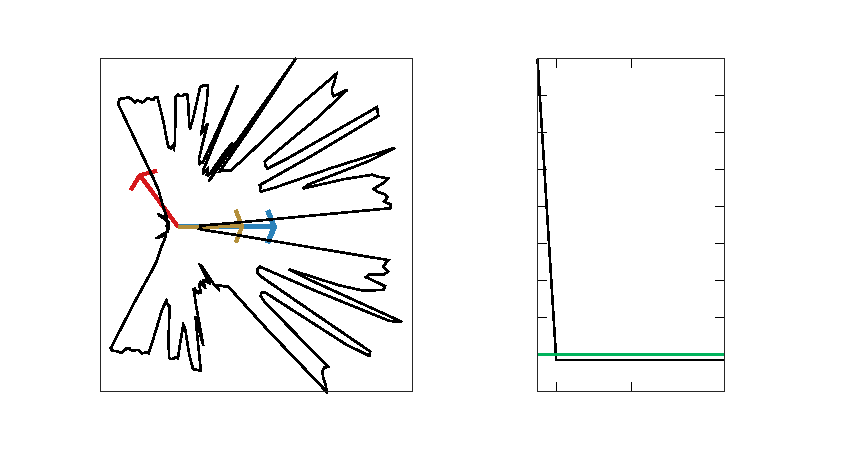
\includegraphics{./figures/parts/02/chapters/04/sections/02/rc_uf}}%
    \gplfronttext
  \end{picture}%
\endgroup

  \vspace{0.5cm}
  \caption{}
  \label{fig:}
\end{figure}


%%%%%%%%%%%%%%%%%%%%%%%%%%%%%%%%%%%%%%%%%%%%%%%%%%%%%%%%%%%%%%%%%%%%%%%%%%%%%%%%
\subsection{Η κλίνη της διακριτικής γωνίας του αισθητήρα}
\label{subsection:02_04_02:04}

Η μέθοδος Fourier-Mellin σε μία διάσταση (ενότητα \ref{subsection:02_04_02:01})
και η μέθοδος του Προκρούστη (ενότητα \ref{subsection:02_04_02:03}), σε
αντίθεση με την μέθοδο πρώτων αρχών (ενότητα \ref{subsection:02_04_02:02}),
είναι διακριτές μέθοδοι εκτίμησης υπό την έννοια ότι λειτουργούν
\textit{μειώνοντας την αρχική εκτίμηση προσανατολισμού κατά ακέραια πολλαπλάσια
της σταθεράς διακριτικής γωνίας $\gamma$}, με αποτέλεσμα αυθαίρετα επίλοιπα
σφάλματα προσανατολισμού $\phi$ όπως ορίζονται από τις παρατηρήσεις
\ref{remark:02_04_02:01} και \ref{remark:02_04_02:03}. Αυτός ο περιορισμός
μπορεί να ιδωθεί ως μία έτερη Προκρούστεια ιδιότητα,\footnote{Στη μυθολογία ο
Πολυπήμων, γνωστότερος ως Προκρούστης, ήταν ένας απαγωγέας ξένων, και μάστιγα
της Ιεράς Οδού της Αττικής. Αφού φιλοξενούσε τα θύματά του προσφέροντάς τούς
ένα πλουσιοπάροχο δείπνο, τα προσκαλούσε να ξαπλώσουν σε ένα κρεβάτι διαστάσεων
τέτοιων που το ύψος του θύματος καλείτο να προσαρμοστεί στο μήκος του
κρεβατιού, είτε μέσω τεμαχισμού του σώματός του, είτε μέσω τάνυσής του. Ο
Πολυπήμων είχε την ατυχία να απαγάγει τον Θησέα, ο οποίος, άρτι αφιχθείς από τη
δολοφονία του Μινώταυρου, τον τιμώρησε χρησιμοποιώντας την τεχνική του εναντίον
τού.} που αφορά σε δύο μεθόδους αυτή τη φορά, υπό την έννοια ότι το αρχικό
σφάλμα προσανατολισμού $|\theta - \hat{\theta}| \in \mathbb{R}_{\geq 0}$
τεμαχίζεται στην κλίνη $K\gamma, K \in \mathbb{Z}_{\geq 0}$, στη βάση διακριτής
και εξωτερικής λογικής:---το αρχικό σφάλμα προσαρμόζεται στη μέθοδο, αντί η
μέθοδος να είναι προσαρμόσιμη στο αρχικό σφάλμα.

Επιπρόσθετα, σύμφωνα με τις παρατηρήσεις \ref{remark:02_04_02:01},
\ref{remark:02_04_02:02}, και \ref{remark:02_04_02:03} τα τελικά σφάλματα
προσανατολισμού των τριών ως άνω μεθόδων εξαρτώνται από τον \textit{αμετάβλητο}
αριθμό των εκπεμπόμενων από τον φυσικό αισθητήρα απόστασης ακτίνων, ή,
ισοδύναμα, από την αμετάβλητη διακριτική του γωνία $\gamma$. Το πεπερασμένο και
αμετάβλητο των εκπεμπόμενων ακτίνων του φυσικού αισθητήρα, σε συνδυασμό με το
αυθαίρετο του ρυθμού των αλλαγών του περιβάλλοντος (σχήμα
\ref{fig:02_02:the_problem}), μπορούν να οδηγήσουν σε υποδειγματοληψία τμημάτων
του περιβάλλοντος ή/και του χάρτη του, με συνέπεια τη μη βέλτιστη σύγκλιση της
εκτίμησης προσανατολισμού.

Οι δύο παραπάνω παρατηρήσεις αφορούν στα σφάλματα στάσης της συνολικής μεθόδου
ευθυγράμμισης, όχι μόνο λόγω των μη επιλύσιμων σφαλμάτων προσανατολισμού αυτών
καθεαυτούς, αλλά και λόγω της διάδοσής τους στην διαδεχόμενη της μεθόδου
ευθυγράμμισης προσανατολισμού μέθοδο ευθυγράμμισης της θέσης (παρατήρηση
\ref{rem:iterative}): λόγω σύζευξης των δύο ειδών ευθυγράμμισης, η μέθοδος
εκτίμησης θέσης απαιτεί επί της αρχής μηδενικά σφάλματα προσανατολισμού. Κατ'
ελάχιστον, όμως, στην περίπτωση των δύο ως άνω Προκρούστειων μεθόδων, το τελικό
σφάλμα προσανατολισμού τους μπορεί να έχει τιμή έως και $\gamma/2$. Για την
επίλυση αυτού του προβλήματος εξετάζουμε δύο υποψήφιες μεθόδους, οι οποίες
παρουσιάζονται στις επόμενες δύο ενότητες.


%%%%%%%%%%%%%%%%%%%%%%%%%%%%%%%%%%%%%%%%%%%%%%%%%%%%%%%%%%%%%%%%%%%%%%%%%%%%%%%%
\subsection{Η μέθοδος του Πιτυοκάμπτη Σίνι}
\label{subsection:02_04_02:05}

Προτού εισάγουμε τη μέθοδο που ελαττώνει τα σφάλματα εκτίμησης προσανατολισμού
που προτείνουμε, πρέπει να εξετάσουμε το λόγο για την πολυπλοκότητά και την
επιτυχία της σε σχέση με την αφελή μέθοδο επιχείρησης ελάττωσης του σφάλματος
εκτίμησης του προσανατολισμού.

Δεδομένων ότι

\begin{itemize}
  \item το τελικό σφάλμα εκτίμησης προσανατολισμού των τριών ως άνω
        μεθόδων είναι αντιστρόφως ανάλογο του αριθμού εκπεμπομένων ακτίνων $N_s$
  \item ο τελευταίος είναι \textit{αμετάβλητος} όσο αφορά στον φυσικό αισθητήρα
        αποστάσεων (με την έννοια ότι δεν μπορεί να προσδώσει περισσότερες
        μετρήσεις από $N_s = 2\pi/\gamma$)
  \item o τελευταίος είναι \textit{μεταβλητός} όσο αφορά στον εικονικό αισθητήρα
        αποστάσεων (με την έννοια ότι, εφόσον οι εικονικές σαρώσεις είναι
        υπολογιστέες μέσω του χάρτη, μπορεί να υπολογιστεί ένας αυθαίρετος
        αριθμός εικονικών ακτίνων εντός του)
\end{itemize}
ο αφελής τρόπος επίλυσης του προβλήματος ελάττωσης του σφάλματος
προσανατολισμού συνίσταται στην αύξηση των εκπεμπόμενων ακτίνων
\begin{itemize}
  \item του φυσικού αισθητήρα με την παρεμβολή των τιμών των ακτίνων της
        πραγματικής σάρωσης
  \item του εικονικού αισθητήρα με την δεσμοβολή ισάριθμων ακτίνων της
        πραγματικής σάρωσης εντός του χάρτη $\bm{M}$
\end{itemize}

Σε αυτή την περίπτωση η αύξηση του αριθμού των ακτίνων της πραγματικής σάρωσης
μέσω παρεμβολής γίνεται με διχοτόμηση όλων των $N_s$ γωνιών μεταξύ γειτονικών
ακτίνων, και εισαγωγή ακτίνων σε γωνίες
$n\gamma + \gamma/2$, $n = 0,1,\dots,N_s-1$, των οποίων η αναφερόμενη απόσταση
τίθεται σε
$\mathcal{S}_R^{\prime\text{\ interp}}[n] = \dfrac{1}{2}(\mathcal{S}_R[n] + \mathcal{S}_R[n+1])$,
όπου $\mathcal{S}_R[N_s] = \mathcal{S}_R[0]$. Με αυτόν τον τρόπο
η προκύπτουσα διακριτική γωνία είναι $\gamma^\prime = \gamma / 2$. Αυτή
διαδικασία θα μπορούσε να επαναληφθεί περαιτέρω, έως ότου η τελική
διακριτική γωνία φτάσει σε ένα αποδεκτά χαμηλό επίπεδο
$\gamma^{(\nu)} = \gamma / 2^\nu$, $\nu \in \mathbb{Z}_{> 0}$. Όσο αφορά στην
εικονική σάρωση, δεδομένου ότι παράγεται από το χάρτη, δεν απαιτεί τη χρήση
παρεμβολής---ο αριθμός των απαιτούμενων εικονικών ακτίνων $N_s^\prime$
καθορίζεται από το μέγεθος της πραγματικής σάρωσης: $N_s^\prime = 2^\nu N_s$.
Λόγω της χρήσης της τεχνικής διχοτόμησης ακτίνων ονομάζουμε αυτή τη μέθοδο ως
μέθοδο του Πιτυοκάμπτη Σίνι.\footnote{Ο Σίνις, επονομαζόμενος Πιτυοκάμπτης, ήταν
γιός του Προκρούστη Πολυπήμωνος. Σε συνέχεια της γενεαλογίας του ο Σίνις απήγαγε
ξένους, των οποίων τα άκρα έδενε σε δύο λυγισμένα πεύκα (κεκαμμένες πιτύες)
προτού αφήσει τα τελευταία να πάρουν τη φυσική τους κλίση, διχοτομώντας έτσι τα
σώματά των θυμάτων του. Για κακή του τύχη εξοντώθηκε επίσης από τον Θησέα.}

\begin{remark}
  \label{rem:sizes_incorrect}
  Κατά τη διάρκεια αυτής της μεθόδου ελάττωσης του σφάλματος προσανατολισμού η
  πραγματική σάρωση και ο χάρτης δειγματοληπτούνται με ρυθμό δειγματοληψίας
  $2^\nu$, με αποτέλεσμα \textit{μία} πραγματική σάρωση και \textit{μία}
  εικονική σάρωση, αποτελούμενες από $2^\nu N_s$ ακτίνες. Η διόρθωση
  προσανατολισμού εκτελείται \textit{μία} φορά, και έχει ως αποτέλεσμα
  \textit{μία} εκτίμηση προσανατολισμού.
\end{remark}

Στο σχήμα \ref{fig:oversampling_goes_wrong} απεικονίζεται μία μεγέθυνση των δύο
περιοχών του σχήματος \ref{fig:02_02:the_problem} που περικλείονται σε κόκκινα
και πράσινα πλαίσια. Η παραπάνω μεθοδολογία υπερδειγματοληψίας προσομοιώνει
τέλεια τις επιπρόσθετες αποστάσεις που θα λάμβανε ένας αισθητήρας με $2^2 N_s$
ακτίνες σε σχέση με έναν αισθητήρα $N_s$ ακτίνων σε γραμμικά τμήματα του
περιβάλλοντος (επάνω σειρά). Όμως, σε μη γραμμικά ή απότομα μεταβαλλόμενα
τμήματα του περιβάλλοντος (κάτω σειρά), η μέθοδος παρεμβολής αστοχεί στην
προσομοίωση των επιπρόσθετων αποστάσεων λόγω εισαγωγής σφαλμάτων απόστασης που
οφείλονται στην επινόηση τεχνητών μετρήσεων. Το μέγεθος αυτών των σφαλμάτων
εξαρτάται από το μέγεθος της διακριτικής γωνίας του αισθητήρα, τον ρυθμό
υπερδειγματοληψίας, και τον χάρτη ως ανεξάρτητη μεταβλητή.

\begin{figure}[h]\centering
  \vspace{0.5cm}
  \definecolor{sr}{RGB}{255,0,0}
\definecolor{sv}{RGB}{0,115,189}
\definecolor{sri}{RGB}{255,0,255}
\definecolor{svi}{RGB}{0,115,189}

% GNUPLOT: LaTeX picture with Postscript
\begingroup
  \makeatletter
  \providecommand\color[2][]{%
    \GenericError{(gnuplot) \space\space\space\@spaces}{%
      Package color not loaded in conjunction with
      terminal option `colourtext'%
    }{See the gnuplot documentation for explanation.%
    }{Either use 'blacktext' in gnuplot or load the package
      color.sty in LaTeX.}%
    \renewcommand\color[2][]{}%
  }%
  \providecommand\includegraphics[2][]{%
    \GenericError{(gnuplot) \space\space\space\@spaces}{%
      Package graphicx or graphics not loaded%
    }{See the gnuplot documentation for explanation.%
    }{The gnuplot epslatex terminal needs graphicx.sty or graphics.sty.}%
    \renewcommand\includegraphics[2][]{}%
  }%
  \providecommand\rotatebox[2]{#2}%
  \@ifundefined{ifGPcolor}{%
    \newif\ifGPcolor
    \GPcolorfalse
  }{}%
  \@ifundefined{ifGPblacktext}{%
    \newif\ifGPblacktext
    \GPblacktexttrue
  }{}%
  % define a \g@addto@macro without @ in the name:
  \let\gplgaddtomacro\g@addto@macro
  % define empty templates for all commands taking text:
  \gdef\gplfronttext{}%
  \gdef\gplfronttext{}%
  \makeatother
  \ifGPblacktext
    % no textcolor at all
    \def\colorrgb#1{}%
    \def\colorgray#1{}%
  \else
    % gray or color?
    \ifGPcolor
      \def\colorrgb#1{\color[rgb]{#1}}%
      \def\colorgray#1{\color[gray]{#1}}%
      \expandafter\def\csname LTw\endcsname{\color{white}}%
      \expandafter\def\csname LTb\endcsname{\color{black}}%
      \expandafter\def\csname LTa\endcsname{\color{black}}%
      \expandafter\def\csname LT0\endcsname{\color[rgb]{1,0,0}}%
      \expandafter\def\csname LT1\endcsname{\color[rgb]{0,1,0}}%
      \expandafter\def\csname LT2\endcsname{\color[rgb]{0,0,1}}%
      \expandafter\def\csname LT3\endcsname{\color[rgb]{1,0,1}}%
      \expandafter\def\csname LT4\endcsname{\color[rgb]{0,1,1}}%
      \expandafter\def\csname LT5\endcsname{\color[rgb]{1,1,0}}%
      \expandafter\def\csname LT6\endcsname{\color[rgb]{0,0,0}}%
      \expandafter\def\csname LT7\endcsname{\color[rgb]{1,0.3,0}}%
      \expandafter\def\csname LT8\endcsname{\color[rgb]{0.5,0.5,0.5}}%
    \else
      % gray
      \def\colorrgb#1{\color{black}}%
      \def\colorgray#1{\color[gray]{#1}}%
      \expandafter\def\csname LTw\endcsname{\color{white}}%
      \expandafter\def\csname LTb\endcsname{\color{black}}%
      \expandafter\def\csname LTa\endcsname{\color{black}}%
      \expandafter\def\csname LT0\endcsname{\color{black}}%
      \expandafter\def\csname LT1\endcsname{\color{black}}%
      \expandafter\def\csname LT2\endcsname{\color{black}}%
      \expandafter\def\csname LT3\endcsname{\color{black}}%
      \expandafter\def\csname LT4\endcsname{\color{black}}%
      \expandafter\def\csname LT5\endcsname{\color{black}}%
      \expandafter\def\csname LT6\endcsname{\color{black}}%
      \expandafter\def\csname LT7\endcsname{\color{black}}%
      \expandafter\def\csname LT8\endcsname{\color{black}}%
    \fi
  \fi
    \setlength{\unitlength}{0.0500bp}%
    \ifx\gptboxheight\undefined%
      \newlength{\gptboxheight}%
      \newlength{\gptboxwidth}%
      \newsavebox{\gptboxtext}%
    \fi%
    \setlength{\fboxrule}{0.5pt}%
    \setlength{\fboxsep}{1pt}%
\begin{picture}(5000.00,5000.00)%
    \gplgaddtomacro\gplfronttext{%
      \put(800,5000){\makebox(0,0){\strut{}{\color{sr}{\rule[0.6mm]{0.5cm}{0.5mm}}}               \small  $\mathcal{S}_R$}}
      \put(1800,5000){\makebox(0,0){\strut{}{\color{sv}{\rule[0.6mm]{0.5cm}{0.5mm}}}              \small  $\mathcal{S}_V$}}
      \put(3300,5000){\makebox(0,0){\strut{}{\color{sri}{\hdashrule[0.6mm]{0.65cm}{0.5mm}{0.5mm}}}\small  $\mathcal{S}_R^{\prime\text{\ interp}}$}}
      \put(4000,5000){\makebox(0,0){\strut{}{\color{svi}{\rule[0.6mm]{0.30cm}{0.5mm}}}}}
      \put(4350,5000){\makebox(0,0){\strut{}{\color{svi}{\hdashrule[0.6mm]{0.35cm}{0.5mm}{0.5mm}}}\small  $\mathcal{S}_V^\prime$}}

      \put(1400,-200){\makebox(0,0){\strut{}\small $|\mathcal{S}_R| = |\mathcal{S}_V| = N_s$}}
      \put(3700,-200){\makebox(0,0){\strut{}\small $|\mathcal{S}_R^\prime| = |\mathcal{S}_R| + |\mathcal{S}_R^{\prime\text{\ interp}}|$}}
      \put(3780,-500){\makebox(0,0){\strut{}\small $= |\mathcal{S}_V^\prime| = 2^2 N_s$}}
    }%
    \gplgaddtomacro\gplfronttext{%
    }%
    \gplgaddtomacro\gplfronttext{%
    }%
    \gplgaddtomacro\gplfronttext{%
    }%
    \gplgaddtomacro\gplfronttext{%
    }%
    \gplgaddtomacro\gplfronttext{%
    }%
    \gplgaddtomacro\gplfronttext{%
    }%
    \gplgaddtomacro\gplfronttext{%
    }%
    \put(0,0){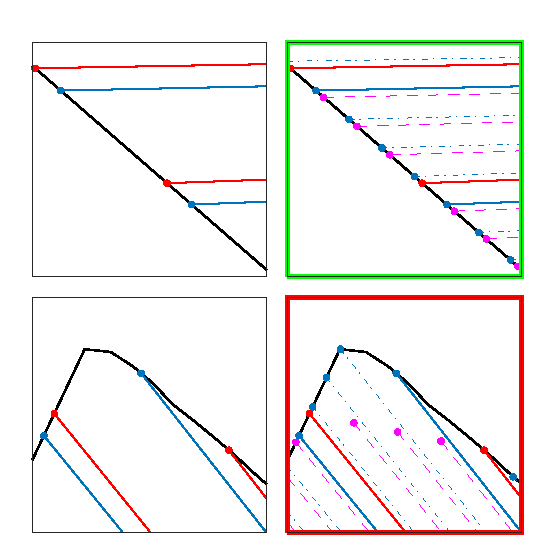
\includegraphics{./figures/parts/02/chapters/04/sections/02/false_oversampling}}%
    \gplfronttext
  \end{picture}%
\endgroup

  \vspace{1.0cm}
  \caption{\small Μεγέθυνση των δύο περιοχών που περικλείονται με κόκκινο
           και πράσινο χρώμα στο σχήμα \ref{fig:02_02:the_problem}. Οι κόκκινες
           γραμμές υποδηλώνουν ακτίνες της πραγματικής μέτρησης $\mathcal{S}_R$.
           Oι μπλε γραμμές υποδηλώνουν ακτίνες της εικονικής μέτρησης $\mathcal{S}_V$.
           Οι διακεκομμένες φούξια γραμμές απεικονίζουν τις παρεμβαλλόμενες
           ακτίνες του πραγματικού αισθητήρα. Οι διακεκομμένες μπλε γραμμές
           απεικονίζουν τις πρόσθετες ακτίνες του εικονικού αισθητήρα.
           Εδώ ο ρυθμός υπερδειγματοληψίας είναι $\mu = 2^\nu$, $\nu = 2$.
           Τα σχήματα στην αριστερή πλευρά δείχνουν τις αρχικές σαρώσεις
           μεγέθους $N_s$. Τα δεξιά σχήματα δείχνουν την παρεμβαλλόμενη
           πραγματική σάρωση και την εικονική σάρωση ίσου μεγέθους $N_s^\prime
           = 2^\nu N_s$. Η παρεμβολή των ακτίνων της πραγματικής σάρωσης είναι
           ακριβής σε γραμμικά τμήματα. Σε μη γραμμικά τµήµατα, όμως, οι
           αποστάσεις των παρεµβαλλόµενων ακτίνων είναι αυθαίρετα λανθασμένες,
           και δεν μπορεί να διασφαλιστεί ότι ο περιορισμός του σφάλματος
           προσανατολισμού κάτω από την τιμή $\gamma/2^{\nu+1}$. }
  \label{fig:oversampling_goes_wrong}
\end{figure}

Αυτό σημαίνει ότι η εισαγωγή παρεμβαλλόμενων ακτίνων έχει το αμετάβλητο και
ακούσιο αποτέλεσμα η λύση να εισάγει τα δικά της σφάλματα στην επιζητούμενη
εκτίμηση. Επιπλέον, αυτό το σφάλμα δεν μπορεί να ελεγχθεί, και, κατά συνέπεια,
είναι αναγκαία εναλλακτική προσέγγιση λύσης του προβλήματος που εκτίθεται στην
ενότητα \ref{subsection:02_04_02:04}.


%%%%%%%%%%%%%%%%%%%%%%%%%%%%%%%%%%%%%%%%%%%%%%%%%%%%%%%%%%%%%%%%%%%%%%%%%%%%%%%%
\subsection{Η μέθοδος του Θησέα}
\label{subsection:02_04_02:06}

Από την παραπάνω ανάλυση γίνεται κατανοητό ότι οποιαδήποτε προσπάθεια
μείωσης του σφάλματος εκτίμησης προσανατολισμού θα πρέπει να περιοριστεί από
την απαγόρευση εφεύρεσης πραγματικών μετρήσεων. Στο σχήμα
\ref{fig:oversampling_correct} απεικονίζεται η μεθοδολογία που εισάγουμε, η
οποία εγγυάται ότι το τελικό σφάλμα προσανατολισμού $|\phi| \in [0,\gamma /
2^{1+\nu}]$ στην περίπτωση που οι μετρήσεις του φυσικού αισθητήρα δεν
διαταράσσονται από θόρυβο και ο χάρτης αναπαριστά το περιβάλλον τέλεια, για
$\nu = 2$.

\begin{figure}[h]\centering
  % GNUPLOT: LaTeX picture with Postscript

\definecolor{BL}{rgb}{0, 0.4470, 0.7410}
\definecolor{OR}{rgb}{0.6500, 0.3250, 0.1980}
\definecolor{GR}{rgb}{0.4660, 0.7740, 0.2880}
\definecolor{PU}{rgb}{0.4940, 0.1840, 0.5560}

\begingroup
  \makeatletter
  \providecommand\color[2][]{%
    \GenericError{(gnuplot) \space\space\space\@spaces}{%
      Package color not loaded in conjunction with
      terminal option `colourtext'%
    }{See the gnuplot documentation for explanation.%
    }{Either use 'blacktext' in gnuplot or load the package
      color.sty in LaTeX.}%
    \renewcommand\color[2][]{}%
  }%
  \providecommand\includegraphics[2][]{%
    \GenericError{(gnuplot) \space\space\space\@spaces}{%
      Package graphicx or graphics not loaded%
    }{See the gnuplot documentation for explanation.%
    }{The gnuplot epslatex terminal needs graphicx.sty or graphics.sty.}%
    \renewcommand\includegraphics[2][]{}%
  }%
  \providecommand\rotatebox[2]{#2}%
  \@ifundefined{ifGPcolor}{%
    \newif\ifGPcolor
    \GPcolorfalse
  }{}%
  \@ifundefined{ifGPblacktext}{%
    \newif\ifGPblacktext
    \GPblacktexttrue
  }{}%
  % define a \g@addto@macro without @ in the name:
  \let\gplgaddtomacro\g@addto@macro
  % define empty templates for all commands taking text:
  \gdef\gplfronttext{}%
  \gdef\gplfronttext{}%
  \makeatother
  \ifGPblacktext
    % no textcolor at all
    \def\colorrgb#1{}%
    \def\colorgray#1{}%
  \else
    % gray or color?
    \ifGPcolor
      \def\colorrgb#1{\color[rgb]{#1}}%
      \def\colorgray#1{\color[gray]{#1}}%
      \expandafter\def\csname LTw\endcsname{\color{white}}%
      \expandafter\def\csname LTb\endcsname{\color{black}}%
      \expandafter\def\csname LTa\endcsname{\color{black}}%
      \expandafter\def\csname LT0\endcsname{\color[rgb]{1,0,0}}%
      \expandafter\def\csname LT1\endcsname{\color[rgb]{0,1,0}}%
      \expandafter\def\csname LT2\endcsname{\color[rgb]{0,0,1}}%
      \expandafter\def\csname LT3\endcsname{\color[rgb]{1,0,1}}%
      \expandafter\def\csname LT4\endcsname{\color[rgb]{0,1,1}}%
      \expandafter\def\csname LT5\endcsname{\color[rgb]{1,1,0}}%
      \expandafter\def\csname LT6\endcsname{\color[rgb]{0,0,0}}%
      \expandafter\def\csname LT7\endcsname{\color[rgb]{1,0.3,0}}%
      \expandafter\def\csname LT8\endcsname{\color[rgb]{0.5,0.5,0.5}}%
    \else
      % gray
      \def\colorrgb#1{\color{black}}%
      \def\colorgray#1{\color[gray]{#1}}%
      \expandafter\def\csname LTw\endcsname{\color{white}}%
      \expandafter\def\csname LTb\endcsname{\color{black}}%
      \expandafter\def\csname LTa\endcsname{\color{black}}%
      \expandafter\def\csname LT0\endcsname{\color{black}}%
      \expandafter\def\csname LT1\endcsname{\color{black}}%
      \expandafter\def\csname LT2\endcsname{\color{black}}%
      \expandafter\def\csname LT3\endcsname{\color{black}}%
      \expandafter\def\csname LT4\endcsname{\color{black}}%
      \expandafter\def\csname LT5\endcsname{\color{black}}%
      \expandafter\def\csname LT6\endcsname{\color{black}}%
      \expandafter\def\csname LT7\endcsname{\color{black}}%
      \expandafter\def\csname LT8\endcsname{\color{black}}%
    \fi
  \fi
    \setlength{\unitlength}{0.0500bp}%
    \ifx\gptboxheight\undefined%
      \newlength{\gptboxheight}%
      \newlength{\gptboxwidth}%
      \newsavebox{\gptboxtext}%
    \fi%
    \setlength{\fboxrule}{0.5pt}%
    \setlength{\fboxsep}{1pt}%
\begin{picture}(5000.00,5000.00)%
    \gplgaddtomacro\gplfronttext{%
    }%
    \gplgaddtomacro\gplfronttext{%
      \colorrgb{0.00,0.00,0.00}%
      \put(1175,4600){\makebox(0,0)[l]{\strut{}$\small \mathcal{S}_R$}}%
      \colorrgb{0.00,0.00,0.00}%
      \put(1175,4349){\makebox(0,0)[l]{\strut{}$\small \mathcal{S}_V^0(\hat{\theta}+0\frac{\gamma}{2^2})$}}%
      \colorrgb{0.00,0.45,0.74}%
      \put(1379,3945){\makebox(0,0)[l]{\color{BL}\strut{}\small $\texttt{PD}^{(2)}_0$$=0.96$}}%
    }%
    \gplgaddtomacro\gplfronttext{%
    }%
    \gplgaddtomacro\gplfronttext{%
      \colorrgb{0.00,0.00,0.00}%
      \put(3625,4600){\makebox(0,0)[l]{\strut{}\small $\mathcal{S}_R$}}%
      \colorrgb{0.00,0.00,0.00}%
      \put(3625,4349){\makebox(0,0)[l]{\strut{}\small $\mathcal{S}_V^1(\hat{\theta}+1\frac{\gamma}{2^2})$}}%
      \colorrgb{0.65,0.33,0.20}%
      \put(3829,3945){\makebox(0,0)[l]{\color{OR}\strut{}\small $\texttt{PD}^{(2)}_1$$=0.90$}}%
    }%
    \gplgaddtomacro\gplfronttext{%
    }%
    \gplgaddtomacro\gplfronttext{%
      \colorrgb{0.00,0.00,0.00}%
      \put(1175,2150){\makebox(0,0)[l]{\strut{}\small $\mathcal{S}_R$}}%
      \colorrgb{0.00,0.00,0.00}%
      \put(1175,1899){\makebox(0,0)[l]{\strut{}\small $\mathcal{S}_V^2(\hat{\theta}+2\frac{\gamma}{2^2})$}}%
      \colorrgb{0.47,0.77,0.29}%
      \put(1379,1495){\makebox(0,0)[l]{\color{GR}\small \strut{}$\texttt{PD}^{(2)}_2$$=0.92$}}%
    }%
    \gplgaddtomacro\gplfronttext{%
    }%
    \gplgaddtomacro\gplfronttext{%
      \colorrgb{0.00,0.00,0.00}%
      \put(3625,2150){\makebox(0,0)[l]{\strut{}\small $\mathcal{S}_R$}}%
      \colorrgb{0.00,0.00,0.00}%
      \put(3625,1899){\makebox(0,0)[l]{\strut{}\small $\mathcal{S}_V^3(\hat{\theta}+3\frac{\gamma}{2^2})$}}%
      \colorrgb{0.49,0.18,0.56}%
      \put(3829,1495){\makebox(0,0)[l]{\color{PU}\small \strut{}$\texttt{PD}^{(2)}_3$$=0.99$}}%
    }%
    \put(0,0){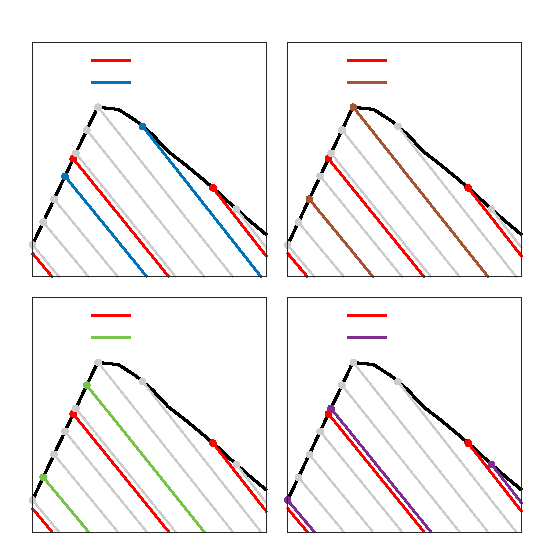
\includegraphics{./figures/parts/02/chapters/04/sections/02/correct_oversampling}}%
    \gplfronttext
  \end{picture}%
\endgroup

  \caption{\small Μεγέθυνση της μη γραμμικής περιοχής που περικλείεται με
           κόκκινο χρώμα στο σχήμα \ref{fig:02_02:the_problem}. Οι κόκκινες
           γραμμές υποδηλώνουν ακτίνες της πραγματικής σάρωσης $\mathcal{S}_R$.
           Οι μπλε, καφέ, πράσινες, και μωβ γραμμές υποδηλώνουν
           ακτίνες $2^\nu = 2^2$ διακριτών εικονικών σαρώσεων που λαμβάνονται
           από την εκτίμηση στάσης $\hat{\bm{p}}(x,y,\hat{\theta})$ σε
           $\gamma/2^\nu$, $\nu = 2$ γωνιακά βήματα, ξεκινώντας από τον
           εκτιμώμενο προσανατολισμό του αισθητήρα $\hat{\theta}$. Η εικονική
           σάρωση που συμβολίζεται με μωβ χρώμα σημειώνει την υψηλότερη τιμή
           της μετρικής Ποσοστού Διάκρισης (PD) μεταξύ όλων των $2^\nu$
           εικονικών σαρώσεων. Χρησιμοποιώντας τη μετρική PD και επιλέγοντας
           την εκτίμηση προσανατολισμού που αντιστοιχεί στην εικονική σάρωση με
           τη μέγιστη τιμή PD, το σφάλμα εκτίμησης προσανατολισμού περιορίζεται
           εγγυημένα κάτω από $\gamma/2^{\nu+1}$ στην περίπτωση όπου οι
           μετρήσεις του φυσικού αισθητήρα δεν διαταράσσονται από θόρυβο και ο
           χάρτης αναπαριστά το περιβάλλον τέλεια}
  \label{fig:oversampling_correct}
\end{figure}

Αντί της κατασκευής μίας εικονικής σάρωσης $2^\nu N_s$ ακτίνων, και της
εκτέλεσης διόρθωσης του προσανατολισμού μία φορά (παρατήρηση
\ref{rem:sizes_incorrect}), το βέλτιστο σφάλμα προσανατολισμού $|\phi| \in
[0,\gamma / 2^{1+\nu}]$ για έναν δεδομένο ρυθμό δειγματοληψίας $\mu = 2^\nu$
και μία διακριτική γωνία $\gamma$ μπορεί να επιτευχθεί με τον υπολογισμό
$2^\nu$ εικονικών σαρώσεων μεγέθους $N_s$, εκτελώντας διόρθωση προσανατολισμού
$2^\nu$ φορές. Η διόρθωση προσανατολισμού πραγματοποιείται μία φορά μεταξύ της
ανόθευτης πραγματικής σάρωσης και της εικονικής σάρωσης $\mathcal{S}_V^k$, η
οποία λαμβάνεται από τη στάση $\hat{\bm{p}}(x,y,\hat{\theta}_k)$:
\begin{align}
  \hat{\theta}_k = \hat{\theta} + k \cdot \gamma / 2^\nu, \ \ \ k = 0,\dots,2^\nu-1 \label{eq:theta_k_theseus}
\end{align}
για συνολικά $2^\nu$ φορές, με αποτέλεσμα $2^\nu$ εκτιμήσεις προσανατολισμού.

Για τη μέθοδο Fourier-Mellin μίας διάστασης και τη μέθοδο του Προκρούστη, η
μετρική ευθυγράμμισης μεταξύ της $k$-οστής εικονικής σάρωσης και της
πραγματικής σάρωσης υπολογίζεται σύμφωνα το Ποσοστό Διάκρισης (Percent
Discrimination---PD). Για τη μέθοδο πρώτων αρχών η σύγκριση ανάμεσα
στις σαρώσεις $\mathcal{S}_R$ και $\mathcal{S}_V^k$ δεν είναι δόκιμη, καθώς
αποτελεί μέθοδο συνεχούς χώρου, και συνεπώς δεν ορίζεται μετρική ευθυγράμμισης.

Η μετρική του Ποσοστού Διάκρισης για την $k$-οστή εικονική σάρωση PD$_k$ $\in
[0,1]$, και είναι ανάλογη του βαθμού ευθυγράμμισης μεταξύ των σαρώσεων
$\mathcal{S}_R$ και $\mathcal{S}_V^k$ για όλες τις $2^\nu$ σαρώσεις
$\mathcal{S}_V^k$. Το Ποσοστό Διάκρισης ανάμεσα στην πραγματική μέτρηση
$\mathcal{S}_R$ και την εικονική σάρωση $\mathcal{S}_V^k$ ορίζεται ως:
\begin{align}
  \text{PD}_k = \dfrac{2 \ F(G,H_k)}{F(G,G) + F(H_k,H_k)} \label{eq:pd}
\end{align}

Για τη μεν περίπτωση της μεθόδου Fourier-Mellin: $F = \max q$, όπου
$q = \mathcal{F}^{-1}\{Q\}$, με τον όρο $Q$ να ορίζεται από την εξίσωση
(\ref{eq:Q0}) με ορίσματα τα διανύσματα σαρώσεων εισόδου $G = \mathcal{S}_R$
και $H_k = \mathcal{S}_V^k$.

Για τη δε περίπτωση της μεθόδου του Προκρούστη: $F = T$, όπου $T$ είναι το
μέγιστο ίχνος με ορίσματα τους πίνακες $G = \bm{P}_R$ και $H_k = \bm{P}_{V_k}$
(επακόλουθο \ref{corollary:umeyama}). Εδώ το σύνολο σημείων $\bm{P}_R$ κατέχει
τις συντεταγμένες των τελικών σημείων των ακτίνων της πραγματικής σάρωσης
$\mathcal{S}_R$ προβεβλημμένες στο επίπεδο $x-y$ από την αρχή $\bm{O}(0,0,0)$
όπως προηγουμένως, και το σύνολο $\bm{P}_{V_k}$ κατέχει τις συντεταγμένες των
τελικών σημείων της $k$-οστής εικονικής σάρωσης, επίσης προβεβλημμένες στο
επίπεδο $x-y$ από το $\bm{O}$.


Έστω τώρα ότι $k_{\max} \in \mathbb{Z}_{\geq 0} : k_{\max} \in [0,2^{\nu-1}]$
συμβολίζει το δείκτη της $k$-οστής εικονικής σάρωσης $\mathcal{S}_V^{k_{\max}}$
που σημειώνει τον υψηλότερο δείκτη ευθυγράμμισης PD$_k$:
$\text{PD}_{k_{\max}} = \max \{\text{PD}_k\}$. Έστω επίσης $I \in \mathbb{Z}$
το ακέραιο πολλαπλάσιο κατά το οποίο εάν πολλαπλασιαστεί η διακριτική γωνία
$\gamma$ τότε η σάρωση $\mathcal{S}_V^{k_{\max}}$ ευθυγραμμίζεται με την
$\mathcal{S}_R$ με τρόπο τέτοιο που παράγεται η μετρική ευθυγράμμισης
PD$_{k_{\max}}$. Τότε εάν η εκτίμηση προσανατολισμού του αισθητήρα ενημερωθεί
σε
\begin{align}
  \hat{\theta}^\prime = \hat{\theta} + I \cdot \gamma + k_{\max} \cdot \dfrac{\gamma}{2^\nu}
\end{align}
το επίλοιπο σφάλμα εκτίμησης προσανατολισμού $\phi$ φράσσεται από:
\begin{align}
  |\phi| = \mod(|\theta - \hat{\theta}^\prime|, \gamma) \leq \dfrac{\gamma}{2^{1+\nu}} < \dfrac{\gamma}{2}
\end{align}
για $\nu \in \mathbb{Z}_{>0}$.

Ο Αλγόριθμος \ref{alg:theseus} παρουσιάζει τη μέθοδο διόρθωσης προσανατολισμού
που προτείνουμε σε μορφή ψευδοκώδικα, για ορίσματα
$\texttt{rc} = \{\texttt{rc\_fm}, \texttt{rc\_uf}\}$.

\begin{algorithm}
  \caption{\texttt{rc\_theseus}}
  \begin{spacing}{1.5}
  \begin{algorithmic}[1]
    \REQUIRE \texttt{rc}, $\bm{M}$, $\mathcal{S}_R$, $\hat{\bm{p}}(x, y, \hat{\theta})$, $\gamma$, $N_s$, $\nu$
    \ENSURE $\hat{\theta}^\prime$
    \STATE $(\hat{\bm{\Theta}}, \textbf{PD}) \leftarrow \texttt{rc\_theseus\_core}(\texttt{rc}, \bm{M}, \mathcal{S}_R, \hat{\bm{p}}(x, y, \hat{\theta}), \gamma, N_s, \nu)$
    \STATE $k_{\max} \leftarrow \arg\max\textbf{PD}$
    \STATE $\hat{\theta}^\prime \leftarrow \hat{\bm{\Theta}}[k_{\max}]$
    \RETURN $\hat{\theta}^\prime$
  \end{algorithmic}
  \end{spacing}
  \label{alg:theseus}
\end{algorithm}

\begin{algorithm}
  \caption{\texttt{rc\_theseus\_core}}
  \begin{spacing}{1.5}
  \begin{algorithmic}[1]
    \REQUIRE \texttt{rc}, $\bm{M}$, $\mathcal{S}_R$, $\hat{\bm{p}}(x, y, \hat{\theta})$, $\gamma$, $N_s$, $\nu$
    \ENSURE $\hat{\bm{\Theta}}$, $\textbf{PD}$
    \STATE $\hat{\bm{\Theta}}, \textbf{PD} \leftarrow \{\varnothing\}$
    \FOR{$k = 0 : 2^\nu-1$}
      \STATE $\hat{\bm{p}}_k \leftarrow (x, y, \hat{\theta} + k \cdot \gamma/2^\nu)$
      \STATE $\mathcal{S}_V^k \leftarrow \texttt{scan\_map}(\bm{M}, \hat{\bm{p}}_k, N_s)$
      \STATE $(\cdot, m_k) \leftarrow \texttt{rc}(\bm{M}, \mathcal{S}_R, \mathcal{S}_V, \hat{\bm{p}}_k, \gamma, N_s)$
      \STATE $\texttt{append} \ \ \hat{\theta}_k = \hat{\theta} + 2\pi m_k/N_s + k \cdot \gamma/2^\nu$ to $\hat{\bm{\Theta}}$
      \STATE $(\cdot,m_k^{R}) \leftarrow \texttt{rc}(\bm{M}, \mathcal{S}_R, \mathcal{S}_R, \hat{\bm{p}}_k, \gamma, N_s)$
      \STATE $(\cdot,m_k^{V}) \leftarrow \texttt{rc}(\bm{M}, \mathcal{S}_V^k, \mathcal{S}_V^k, \hat{\bm{p}}_k, \gamma, N_s)$
      \STATE $\texttt{append} \ \ \dfrac{2m_k}{m_k^{R} + m_k^{V}}$ to \textbf{PD}
      \STATE $k \leftarrow k + 1$
    \ENDFOR
    \RETURN $(\hat{\bm{\Theta}}, \textbf{PD})$
  \end{algorithmic}
  \end{spacing}
  \label{alg:core_theseus}
\end{algorithm}

\begin{algorithm}
  \caption{\texttt{scan\_map}}
  \begin{spacing}{1.3}
    \begin{algorithmic}[1]
      \REQUIRE $\bm{M}, \bm{p}(x, y, \theta), N_s$
      \ENSURE $\mathcal{S}_V$
      \STATE $\mathcal{S}_V \leftarrow \{\varnothing\}$
      \FOR{$n = 0:N_s-1$}
      \STATE $\lambda_n \leftarrow -\pi + \dfrac{2\pi}{N_s} n$
      \STATE $\theta_n \leftarrow \lambda_n + \hat{\theta}$
      \STATE $(x_n,y_n) \leftarrow \texttt{intersect}(\bm{M}, (x,y, \theta_n))$
      \STATE $d_n \leftarrow \|(x- x_n, y-y_n)\|_2$
      \STATE \texttt{append} $(d_n, \lambda_n)$ to $\mathcal{S}_V$
      \ENDFOR
      \RETURN $\mathcal{S}_V$
    \end{algorithmic}
  \end{spacing}
  \label{alg:scan_map}
\end{algorithm}

Ο στόχος (\ref{objective:02_04}) ?? επιτυγχάνεται με τη μέθοδο που εισαγάγαμε σε
αυτή την ενότητα για τη μέθοδο Fourier-Mellin μίας διάστασης (ενότητα
\ref{subsection:02_04_02:01}) και τη μέθοδο του Προκρούστη (ενότητα
\ref{subsection:02_04_02:03}) υπό τις προϋποθέσεις ότι (α)
$\bm{l} = \hat{\bm{l}}$, και (β) το αρχικό σφάλμα προσανατολισμού είναι
$|\theta - \hat{\theta}| > \gamma / 2^{1+\nu}$ για δεδομένο βαθμό
δειγματοληψίας $\nu$.
